\documentclass[]{book}
\usepackage{lmodern}
\usepackage{amssymb,amsmath}
\usepackage{ifxetex,ifluatex}
\usepackage{fixltx2e} % provides \textsubscript
\ifnum 0\ifxetex 1\fi\ifluatex 1\fi=0 % if pdftex
  \usepackage[T1]{fontenc}
  \usepackage[utf8]{inputenc}
\else % if luatex or xelatex
  \ifxetex
    \usepackage{mathspec}
  \else
    \usepackage{fontspec}
  \fi
  \defaultfontfeatures{Ligatures=TeX,Scale=MatchLowercase}
\fi
% use upquote if available, for straight quotes in verbatim environments
\IfFileExists{upquote.sty}{\usepackage{upquote}}{}
% use microtype if available
\IfFileExists{microtype.sty}{%
\usepackage{microtype}
\UseMicrotypeSet[protrusion]{basicmath} % disable protrusion for tt fonts
}{}
\usepackage[margin=1in]{geometry}
\usepackage{hyperref}
\hypersetup{unicode=true,
            pdftitle={Teaching and Learning with Jupyter},
            pdfborder={0 0 0},
            breaklinks=true}
\urlstyle{same}  % don't use monospace font for urls
\usepackage{natbib}
\bibliographystyle{apalike}
\usepackage{longtable,booktabs}
\usepackage{graphicx,grffile}
\makeatletter
\def\maxwidth{\ifdim\Gin@nat@width>\linewidth\linewidth\else\Gin@nat@width\fi}
\def\maxheight{\ifdim\Gin@nat@height>\textheight\textheight\else\Gin@nat@height\fi}
\makeatother
% Scale images if necessary, so that they will not overflow the page
% margins by default, and it is still possible to overwrite the defaults
% using explicit options in \includegraphics[width, height, ...]{}
\setkeys{Gin}{width=\maxwidth,height=\maxheight,keepaspectratio}
\IfFileExists{parskip.sty}{%
\usepackage{parskip}
}{% else
\setlength{\parindent}{0pt}
\setlength{\parskip}{6pt plus 2pt minus 1pt}
}
\setlength{\emergencystretch}{3em}  % prevent overfull lines
\providecommand{\tightlist}{%
  \setlength{\itemsep}{0pt}\setlength{\parskip}{0pt}}
\setcounter{secnumdepth}{5}
% Redefines (sub)paragraphs to behave more like sections
\ifx\paragraph\undefined\else
\let\oldparagraph\paragraph
\renewcommand{\paragraph}[1]{\oldparagraph{#1}\mbox{}}
\fi
\ifx\subparagraph\undefined\else
\let\oldsubparagraph\subparagraph
\renewcommand{\subparagraph}[1]{\oldsubparagraph{#1}\mbox{}}
\fi

%%% Use protect on footnotes to avoid problems with footnotes in titles
\let\rmarkdownfootnote\footnote%
\def\footnote{\protect\rmarkdownfootnote}

%%% Change title format to be more compact
\usepackage{titling}

% Create subtitle command for use in maketitle
\newcommand{\subtitle}[1]{
  \posttitle{
    \begin{center}\large#1\end{center}
    }
}

\setlength{\droptitle}{-2em}

  \title{Teaching and Learning with Jupyter}
    \pretitle{\vspace{\droptitle}\centering\huge}
  \posttitle{\par}
    \author{Lorena A. Barba, Lecia J. Barker, Douglas Blank, Jed Brown, Allen
Downey, Tim George, Lindsey Heagy, Kyle Mandli, Jason K. Moore, David
Lippert, Kyle E. Niemeyer, Ryan Watkins, Richard West, Elizabeth Wickes,
Carol Willing, and Michael Zingale}
    \preauthor{\centering\large\emph}
  \postauthor{\par}
      \predate{\centering\large\emph}
  \postdate{\par}
    \date{2018-11-30}

\usepackage{booktabs}
\usepackage{amsthm}
\makeatletter
\def\thm@space@setup{%
  \thm@preskip=8pt plus 2pt minus 4pt
  \thm@postskip=\thm@preskip
}
\makeatother

\begin{document}
\maketitle

{
\setcounter{tocdepth}{1}
\tableofcontents
}
\chapter{Introduction}\label{intro}

Project Jupyter is a broad collaboration that develops open-source tools
for interactive and exploratory computing. The tools include: IPython,
the Jupyter Notebook, Jupyter Hub, and an ecosystem of extensions
contributed by a large community. Jupyter Notebook exploded in
popularity since late 2014, fueled by its adoption as the favorite
environment for doing data science. It has also grown as a platform to
use in the classroom, to develop teaching materials, to share lessons
and tutorials, and more. Notebooks are documents containing text
narratives, combined with executable code (many languages are supported)
and the output of that code. This marriage of content and code makes for
a powerful new form of data-based communication. Educators everywhere
are adopting Jupyter for teaching.

This handbook is for any educator teaching a topic that includes data
analysis or computation to support the learning---not just courses in
engineering or science, but also data journalism, business and
quantitative economics, data-based decision sciences and policy,
quantitative health sciences, and others. It aims to give an entry
point, and a broad overview of Jupyter in education. Whether you are
already using Jupyter to teach, you have found learning materials built
on Jupyter that piqued your curiosity, or have never heard of Jupyter,
the material in this open book can help you empower your teaching with
this new technology.

Educators newly adopting Jupyter can be overwhelmed by having to
navigate the ecosystem of tools and content. They could study many
examples, or consume myriad blog posts and talk videos to distill the
patterns of good practices and technical solutions to best serve their
students. Several early adopters, having much experience to share,
decided to begin collecting this know-how, and sharing open
documentation about using Jupyter for teaching and learning.

The Jupyter Community Workshop in DC (November 2018) began that process,
with a book sprint aimed at producing the first version of this
handbook. The collaboratively written book consolidates explanations and
examples covering key topics, including: what is Jupyter, how to try
Jupyter, sharing notebooks with students, locally installing Jupyter,
cloud offerings, finding example notebooks, writing lessons in Jupyter,
making collections for a course, exporting to other formats with
nbconvert, writing textbooks with Jupyter, using Binder, JupyterHub,
making assignments and auto-grading, making online courses, teaching
with Jupyter in the classroom, active learning and flipped learning
pedagogies with Jupyter, guiding learners to create their own content in
Jupyter, and more. This open handbook will grow to encompass all you
need to know about Jupyter in Teaching and Learning.

If you find these materials helpful or inspiring, give us a shout-out on
Twitter using \#Jupyter4Edu. We hope you do!

\textbf{Acknowledgements}

The book sprint was held at the George Washington University in
Washington, DC, on 28--30 November 2018, and organized by Lorena A.
Barba. Funding to support the logistics and travel of all participants
was possible thanks to a grant from Bloomberg to Project Jupyter, and
managed by NumFOCUS. The group was fêted at a reception sponsored by
Leidos. Participants traveled from all over the country and volunteered
their precious time and hard work to give this work to the Jupyter
community, with a heartfelt sense of gratitude to all the contributors
to the software projects we love and depend on. Thank you!

GitHub repository for this book:
\url{https://github.com/jupyter4edu/jupyter-edu-book}

\chapter{Why we use Jupyter
Notebooks}\label{why-we-use-jupyter-notebooks}

\section{Introduction}\label{introduction}

In Chapter 2, you will be introduced to why and how educators are using
Jupyter Notebooks. We will highlight examples illustrating how notebooks
are being used to increase student engagement, participation,
understanding, and performance. Notebooks can also have benefits for
students that extend beyond your course, while also offering substantial
benefits to you, the teacher, over other tools.

\section{Why do we as educators use
Jupyter?}\label{why-do-we-as-educators-use-jupyter}

As teachers we are responsible for a vast array of activities, including
creating lessons, lectures, courses, assignments, and supportive
environments; encouraging engagement and performance in the classroom;
helping students learn to think critically so they can become lifelong
learners and problem solvers; making material relevant and meaningful to
students' diverse interests and backgrounds; assessing student learning
(including grading and evaluation); encouraging students to persist with
emotional labor (feedback, communication, etc.); and trying out teaching
and learning practices that improve our ability to do all of these
things.

In short, teachers design learning environments and experiences. We use
Jupyter Notebooks to design learning environments to help support these
activities. The goal of this handbook is to provide you with ideas to
help you address your own instructional and pedagogical goals. We
believe that incorporating Jupyter Notebooks in our teaching has allowed
us to help improve students' understanding of course content, help
increase student engagement and participation in class, and help make
concepts more meaningful and relevant to students' diverse interests. We
have found that this can be achieved in a variety disciplines and across
many diverse types of instructional goals.

Through a series of anecdotes we will illustrate how you, as an
educator, can help increase your students' 1) engagement, 2)
participation, 3) understanding, 4) performance, 5) preparation for
their career, using Jupyter notebooks. These are starting places and we
are confident that you will also take these examples in new and exciting
directions.

\section{But first, what is Jupyter
Notebook?}\label{but-first-what-is-jupyter-notebook}

Project Jupyter is three things: a collection of standards, a community,
and a set of software tools. Jupyter Notebook is software that creates a
notebook, is a document that supports mixing executable code, equations,
visualizations, and narrative text. Jupyter notebooks allow a user to
bring together data, code, and prose to tell an interactive,
computational story. Whether analyzing a corpus of American Literature,
creating music and art, or illustrating the engineering concepts behind
Digital Signal Processing, a notebook can combine explanations
traditionally found in textbooks, but with \emph{the interactivity of an
application}.

Figure

Visual of a notebook - Side Box with an anatomy of a notebook -
descriptions with arrows to particular cells. Link to Binder: Try it
now.

Title Cell: Point out prose (markdown)

Introduction Cell: Links to other content

Engaging visualization (a few lines of code 5 or less)

Make the example interactive with widgets

Add a cell with a problem to solve

Solution cell

It would be nice also to have a callout box here that illustrates a
relatively simple use of JN for say, one learning objective -- or maybe
one of each of the following: domain knowledge, programming, and other
use.

Jupyter Notebook is a free, open source platform that is an excellent
learning environment for students. For teachers, it increases our
efficiency and decreases cognitive load so we can spend our time
engaging students. Notebooks can be useful for achieving your goals as a
teacher in numerous environments from STEM labs or humanities
narratives, to podium lectures or flipped classrooms. We use Jupyter
Notebook in small classes and for classes that have hundreds of
students. Jupyter Notebook can be used for teaching part of one lecture
or can be used to teach a whole course. Jupyter Notebook enables us and
our students to have a conversation with a problem and link to
resources, like audio, video, images, visualizations--and even allow
students to mix and remix these. \emph{And yet students need to install
nothing beyond a modern web browser to use this free software.}

Jupyter Notebook can be used to organize classroom materials and
objects, store and provide access to reading materials for students,
present and share lecture materials, perform live coding, explore and
interact with materials, support self-paced learning, grade students'
homework, solve homework problems, and make materials reusable to others
( TODO see Chapters 3 and 4).

Read on to find out how we have used Jupyter Notebooks for teaching and
learning to benefit both our students and ourselves.** **Jupyter
Notebook support a wide range of learning goals, including learning to
program, learning domain knowledge, and practicing communication skills
like storytelling. The authors of this book have used Jupyter Notebook
to teach:

\begin{itemize}
\tightlist
\item
  Sciences

  \begin{itemize}
  \tightlist
  \item
    Physics and astronomy
  \item
    Geoscience
  \item
    Biology
  \item
    Cognitive Science
  \item
    Computer science
  \item
    Data science
  \item
    Statistics
  \item
    Social sciences
  \end{itemize}
\item
  Writing

  \begin{itemize}
  \tightlist
  \item
    Writing Seminar
  \item
    Writing and technical communication
  \end{itemize}
\item
  Digital Humanities

  \begin{itemize}
  \tightlist
  \item
    Music
  \item
    Text analysis
  \item
    Metadata processing
  \end{itemize}
\item
  Engineering

  \begin{itemize}
  \tightlist
  \item
    Chemical engineering (kinetics and reactor design)
  \item
    Mechanical engineering
  \item
    Aerospace engineering
  \end{itemize}
\item
  Introduction to Programming

  \begin{itemize}
  \tightlist
  \item
    High school
  \item
    College and university-level courses (true introductions through
    advanced courses)
  \end{itemize}
\end{itemize}

Our other use of notebooks for education include:

\begin{itemize}
\tightlist
\item
  Building models/simulations (with and without programming)
\item
  Using widgets to demonstrate and interact with simulations
\item
  Visualizations of process and data
\end{itemize}

\section{Course Benefits \& Anecdotes}\label{course-benefits-anecdotes}

\subsection{Engagement}\label{engagement}

As teachers we routinely struggle to engage our students, especially
when we are constrained by the format of the course (e.g., online,
50-minute lecture), available technologies, students distractions,
and/or other factors. Nevertheless, it is substantially our
responsibility to create environments and experiences within these
limits that engage students in our courses. This is where notebooks can
give you another tool to break out of the mundane, and get students
engaged in their learning.

\subsubsection{Conversations with Data}\label{conversations-with-data}

The creators of Jupyter describe it as a set of open-source tools for
interactive and exploratory computing, and a platform for creating
computational narratives. Jupyter allows us, as educators, to narrate a
``conversation between the student and data''. Consider this example,
using the data of life expectancy of many countries over the years:

\begin{verbatim}
_I use a short bit of code to make a graph showing the time evolution, in what is called a "spaghetti plot" (see figure). Looking at this messy graphic, I point out how most of the lines show growth over time: life expectancy is improving all over the world. But a couple of lines show a marked dip in a given year. I can ask students: which country had that dip? What happened there? Why? With a bit more coding, we identify that Cambodia had a shocking life expectancy of about 30 years in 1977, and Rwanda had even worse life expectancy in 1992. We then have the opportunity to discuss why these countries experienced a mortality crisis. The data brings to life a meaningful discussion, with many possible paths involving history, politics, economics, and health. -- Lorena Barba_
\end{verbatim}

\begin{figure}
\centering
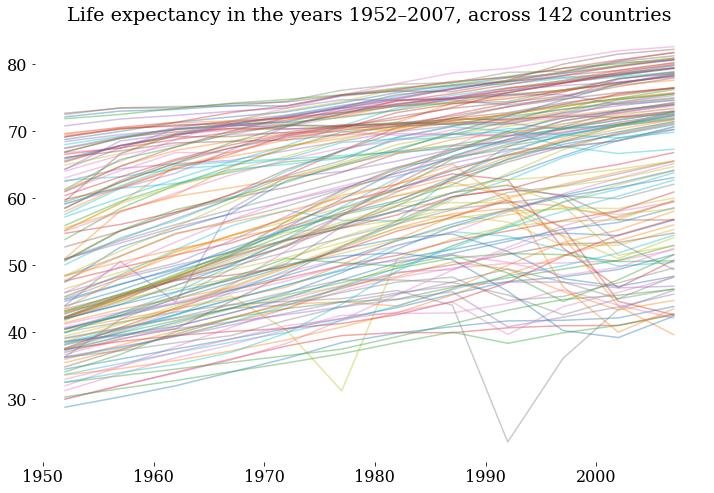
\includegraphics{figures/engcomp2lesson4-life-expectancy.png}
\caption{From: \url{http://go.gwu.edu/engcomp2lesson4}}
\end{figure}

Jupyter notebooks are essential tools of connection -- tools that engage
learners in transitions in their thinking. The opportunity of
intermingling computation into a narrative, creating a conversation with
data is a powerful and effective form of communication. With Jupyter,
you now have a new form of content to create and share with learners:
\emph{computable content}. In a world where every subject matter can
have a data-supported treatment, where computational devices are
omnipresent and pervasive, the union of natural language and computation
creates compelling communication and learning opportunities.

\subsection{Participation}\label{participation}

Engaging students in your courses requires their participation and
interaction with you, their peers, and/or the content {[}Michael Moore,
1989{]}. How, when, and why you use student participation in yours will,
of course, depend on your goals, the specific objectives for teaching
the content within your course, your students, and other factors. Using
notebooks, however, encourages participation and gives you more tools
for promoting participation. Notebooks can connect students to authentic
external audiences as well. Students can, for example, consume notebooks
from other classes, and publish notebooks where others can read them.

\subsubsection{Real World Experience -- bringing concepts to
life}\label{real-world-experience-bringing-concepts-to-life}

Notebooks are living documents, meaning they can be edited to respond to
questions or input from students and used a conversation piece during a
lecture or presentation.

\begin{verbatim}
_Our group uses Jupyter notebooks as "apps" to demonstrate concepts in geophysics. These notebook-apps connect numerical simulations to widgets and relevant plots. In the classroom, we ask students to help define input parameters based on an application or case study that they are interested in. Prior to displaying the results, we ask students to build a mental image of their expectations. If the resultant image matches their expectations, then we have reinforced a concept, and if not, it is an opportunity to learn. We as instructors can interactively engage with students' questions by updating the inputs to the simulation in order to explore concepts with them. Students have access to the same notebooks through free web-platforms like Binder, so simply by following a link, they can take the steering wheel and engage with the concepts on their own. Notebooks bring the concepts to life and serve as a conversation piece for the interaction between learners and educators. -- Lindsey Heagy_
\end{verbatim}

\begin{figure}
\centering
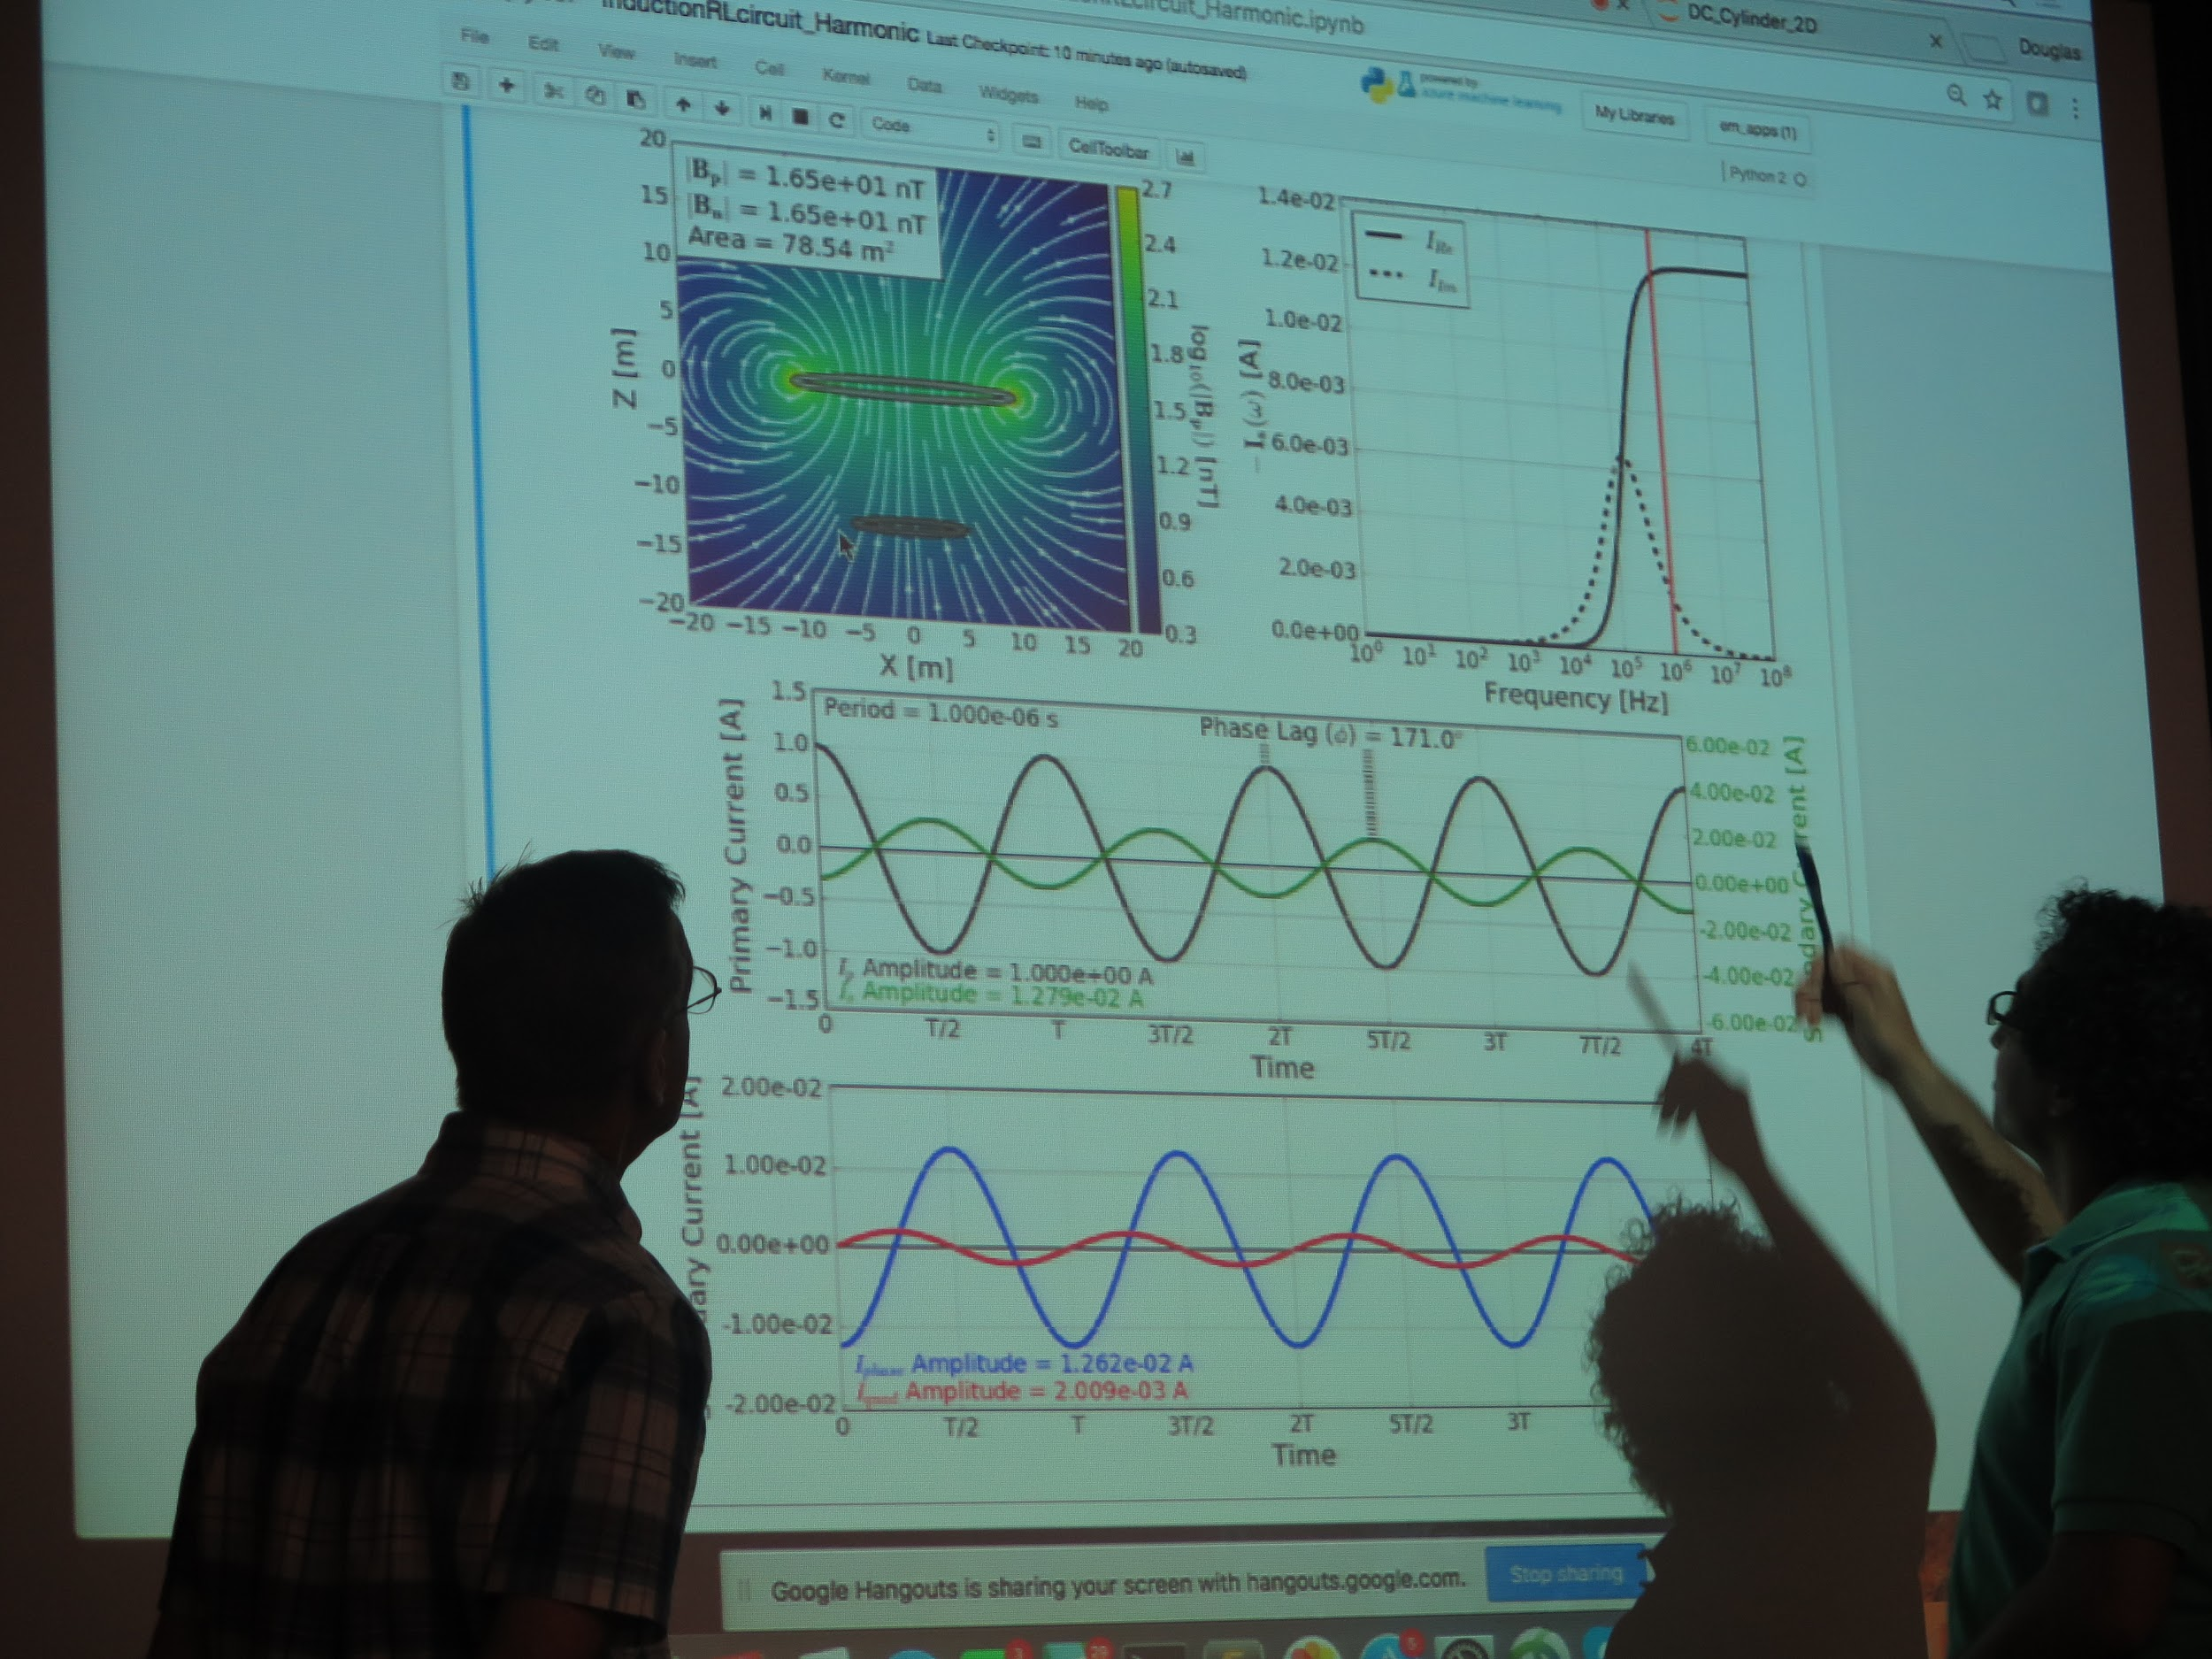
\includegraphics{figures/oldenburg-geosci.jpg}
\caption{Dr.~Douglas Oldenburg (left) engaging with a student during a
short course on geophysical electromagnetics (\url{https://geosci.xyz}).
Photo credit: Seogi Kang}
\end{figure}

\subsubsection{Real World Experience -- Ticket to
leave}\label{real-world-experience-ticket-to-leave}

Another example of generating participation in the classroom with
Jupyter notebooks is the Activity magic, available as an extension. It
creates what has been called a ``ticket to leave'' (or ``exit ticket'')
via the notebook. The idea of a ``ticket to leave'' is an excellent way
to end a class or lab. Briefly, it is just a survey that you give the
students (see figure). Often, these surveys are given via a Personal
Response System (also known as ``clickers'' or PRS) or cell phones.
There are a few uses of such surveys:

\begin{enumerate}
\def\labelenumi{\arabic{enumi}.}
\tightlist
\item
  Give the instructor some feedback on the students' understanding, as a
  whole
\item
  Provide time and opportunity for students to review and synthesize
  today's materials
\item
  Allow the students to apply their recent knowledge to a novel problem
\item
  An additional instance to learn the materials
\end{enumerate}

\begin{figure}
\centering
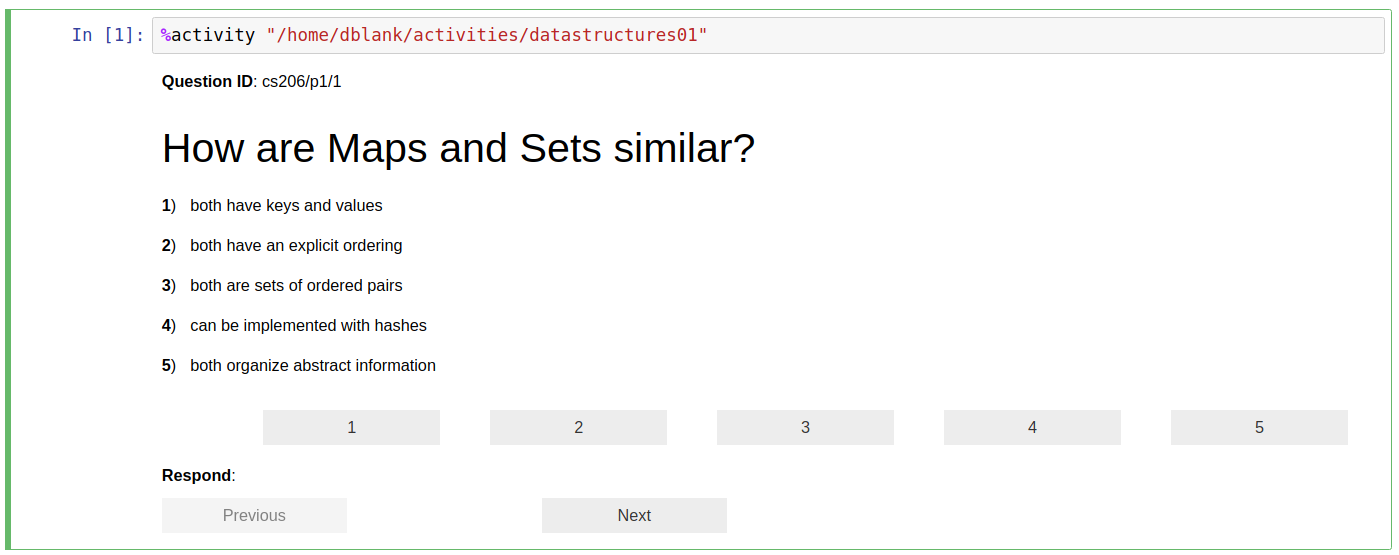
\includegraphics{figures/activity-magic-student.png}
\caption{Example of the Activity magic seen from the students view. A
question, with multiple choice answers is shown, with buttons for their
input.}
\end{figure}

These questions do not typically require much time to answer, but are
meant to capture the essence of the conversation of the class. After a
minute or so to contemplate the question, the students select their
answer (by clicking one of the buttons), and instructor shows the
gestalt results (see figure).

\begin{figure}
\centering
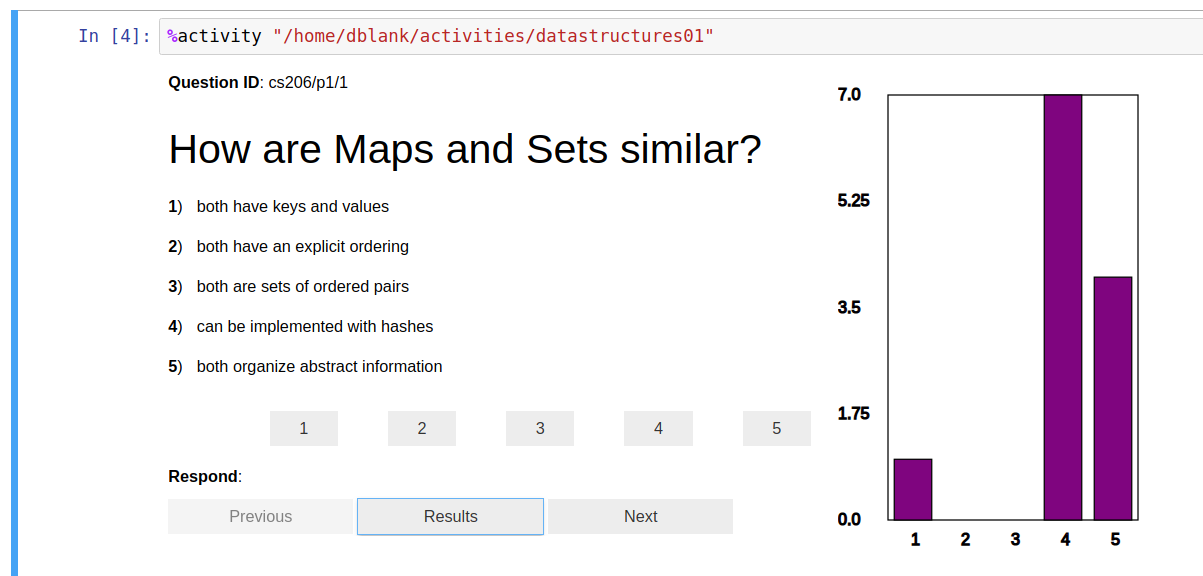
\includegraphics{figures/activity-magic-instructor.png}
\caption{The Activity magic, from the the instructor's perspective. The
barchart is shown on the project once all of the students have had a
chance to respond.}
\end{figure}

Good ``exit ticket'' questions can be domain specific questions, but can
also be metacognitive questions (about one's learning style, for
example), or high-level organizational questions (e.g., ``what was the
goal of today's discussion?''). We recommend leaving enough time at the
end of class (perhaps 10 minutes) to have a full and complete wrap-up
discussion. After the discussion, you may wish to adjust the following
class meeting if you feel that not enough students had the insight you
were aiming for. For more information on ``tickets to leave'' see
\url{https://www.brown.edu/sheridan/teaching-learning-resources/teaching-resources/course-design/classroom-assessment/entrance-and-exit/sample}

\subsection{Increasing Understanding}\label{increasing-understanding}

Within any course you will typically try to achieve a diverse set of
objectives. Benjamin Bloom
(\url{https://en.wikipedia.org/wiki/Bloom\%27s_taxonomy}) provided a
framework for the detailed objectives we want to achieve, ranging from
basic knowledge (such as, terminology, specific facts, trends and
sequences, classifications and categories, etc.) all the way to ability
to evaluate and create (such as, abstract relationships, judgments but
based criteria, original works). Achieving the former (i.e., basic
knowledge and comprehension) is far easier to achieve that understanding
(i.e., evaluation and creation); yet, most often we, as educators, are
striving for increasing the complex understanding of our students on the
topics we are teaching. The good news is that notebooks offer a valuable
tool for teaching toward understanding -- moving students, for example,
from passively viewing course content to exploring, analyzing,
synthesizing, and evaluating the content in active ways.

\subsubsection{Real World Experience -- Guiding Learners at their Own
Pace}\label{real-world-experience-guiding-learners-at-their-own-pace}

The fundamental theory behind Computational Fluid Dynamics (CFD) used in
Aerospace Engineering is based on understanding the Navier-Stokes
equations. ``CFD Python'' is a collection of Jupyter Notebooks based on
a practical module that I began using in class in my Computational Fluid
Dynamics (CFD) course at Boston University in 2009. The 5-week module
develops worked examples that build on each other to incrementally guide
the learner to create a program to solve the Navier-Stokes equations of
fluid mechanics, in 12 steps.

\begin{verbatim}
_In 2013, I was invited to teach a 2 day mini-course in the Latin-American School in High-Performance Computing, in Argentina. The Jupyter Notebooks platform allowed me to create a guided narrative to support learners with different background experience and knowledge. For that event, we wrote Notebooks based on the CFD course module, to use as instructional scaffolding in the minicourse. Twenty students worked through the notebooks as self-paced lessons, while I went from desk to desk asking and answering questions. About four of the students completed all 12 steps in the 2 days, a bulk of them achieved up to about Step 8, and a few of them lagged behind in Steps 4 or 5 by the end of the course. For those who completed the full module, they had achieved in 2 days what my regular students in the classroom normally took 5 weeks to do. Seeing that was an eye-opening moment: both the power of worked examples in code, and the ability to allow learners to follow their own pace made a remarkable difference in these learners. -- Lorena Barba_
\end{verbatim}

Based on the experience developing the ``CFD Python'' learning module
{[}\emph{Barba et. Al 2018 }\url{https://doi.org/10.21105/jose.0002}{]},
this basic design pattern was adopted for creating lessons using
computable content:

\begin{enumerate}
\def\labelenumi{\arabic{enumi}.}
\tightlist
\item
  Break it down into small steps
\item
  Chunk small steps into bigger steps
\item
  Add narrative and connect
\item
  Link out to documentation
\item
  Interleave easy exercises
\item
  Spice with challenge questions/tasks
\item
  Publish openly online
\end{enumerate}

This was particularly helpful for student understanding.

\subsection{Increasing Student's
Performance}\label{increasing-students-performance}

The goal of learning is often actualized through the performance of
students. This is routinely most visible by what we attempt to assess
during and at the end of instruction. Using notebooks we can create a
variety of a performance opportunities for students, thereby giving them
more opportunities for practice and feedback, as well as more
opportunities for us, as instructors, to assessment their ability to
perform.

\subsubsection{Real World Experience -- The Worked-example
effect}\label{real-world-experience-the-worked-example-effect}

The worked-example effect is the best known and most widely studied of
the cognitive load effects {[}Sweller, J. (2006){]}. It refers to
providing full guidance on how to solve a problem, resulting in better
student performance than problem-solving conditions with no guidance.
For complex tasks, inexperienced or beginner learners benefit the most
from the worked-examples procedure. One study (Chen et al., 2015)
concludes that: ``worked example effect occurs for complex, high-element
interactivity materials that impose a heavy working memory load'' and
``when dealing with complex material that learners may have difficulty
understanding, high levels of guidance are likely to result in enhanced
performance over lower levels of guidance.'' This research-based
guidance seems especially relevant for teaching novice programmers to
use computation in the context of their subject matter (science,
engineering, or other).

\subsection{Increasing Students' Preparation for Their
Career}\label{increasing-students-preparation-for-their-career}

In preparing students to apply what they have learned, striving to align
what happens in the course with what they will experience in their
career is important. From using parallel software to mirroring
workflows, we want our students to experience and be prepared for the
workplace. Recognizing, of course, that workplaces are not static and
the skills required for a career are always emerging, using notebooks
provides a flexible platform to build skills and build portfolios of
what students can do.

\subsubsection{Real World Experience -- Publishing a data narrative as a
demonstration of industry
ability}\label{real-world-experience-publishing-a-data-narrative-as-a-demonstration-of-industry-ability}

For Data Science careers, a publicly shared narrative about a data
analytics project goes a long way at demonstrating the student's
potential at an interview. Elizabeth Wicks has her students develop a
Jupyter notebook that tells the story of a data munging and analysis
project done in the class. The students then publish this notebook to
their Github profile pages. Being that Jupyter is one of the most
popular ways in industry to communicate data science results, the
students have a very valuable key to a potential career.

TODO: Add quote from Elizabeth

\section{Student benefits}\label{student-benefits}

Creating opportunities for students to develop as learners stretch
beyond the boundaries of any specific course where you may use
notebooks. By enriching their learning experience in your course, you
will help them develop valuable skill-sets and mind-sets that they will
take with them into other courses and into their career.

\subsection{Computational Thinking}\label{computational-thinking}

Jupyter Notebooks support a wide range of learning goals. Its
interactivity enables building intuitive understanding of domain
knowledge, such as the understanding of a mechanical response of a
system while varying parameters or understanding how an algorithm
behaves. Notebooks can also help teach effective communication skills,
combining prose with graphics into a strong narrative. Finally,
notebooks can support teaching or strengthening programming skills, by
combining code with text descriptions and visualizations. Even if a
notebook is designed to be consumed passively, the exposure to code
helps show students how to do something---and that they can do it
themselves. This also helps demystify coding for students who do not
view themselves as traditional ``computer science'' types.

Using notebooks, you can create rich learning experiences that link
together the core foundations of computational thinking:

\begin{itemize}
\tightlist
\item
  \emph{Decomposition}: Breaking down data, processes, or problems into
  smaller, manageable parts
\item
  \emph{Pattern Recognition}: Observing patterns, trends, and
  regularities in data
\item
  \emph{Abstraction}: Identifying the general principles that generate
  these patterns
\item
  \emph{Algorithm Design}: Developing the step by step instructions for
  solving this and similar problems (see
  \url{https://usr55.dayforcehcm.com/CandidatePortal/en-US/myeyedr/Posting/View/8612?fbclid=IwAR0BVRfn38L7PMftCSbYY_n7IZDhMba0HA7Mmn78ASu5rRIivvPtcAYqxWs})
\end{itemize}

\subsection{Open-source}\label{open-source}

Integrating notebooks into classes also exposes students to a large and
growing ecosystem of open-source tools. This supports their education,
but also provides experience in the same environment of tools used in
industries in high demand for trained employees, such as data science
and machine learning. The open-source nature of these tools also ensures
that course content remains accessible and affordable to all
students---including those outside the traditional university
environment.

Unlike proprietary notebook technologies such as Mathematica, or
specific programming languages/environments such as Matlab or C++, the
barriers to entry for students learning with Jupyter notebooks can be
extremely low. At a minimum, during a lecture, students can simply
watch/read an interactive demo using a notebook, to replace slides or
lecture notes. On their own, using a cloud service such as Binder or
JupyterHub, students can open any modern web browser to some address and
interact with a notebook (an example of this technology can be found at
\url{https://jupyter.org/try}) , without needing any installation or
configuration. In the most complicated case, students can install
Anaconda and follow simple instructions to install the Jupyter Notebook,
which works and looks the same on all platforms---and is free and open
source.

\subsection{Active learning}\label{active-learning}

Thanks to their interactivity, notebooks enable a spectrum of active
learning methods, which have been shown to increase performance in
science, engineering, and mathematics {[}Freeman et al. 2018{]}. To
start, students can consume notebook content by reading and running
notebooks, then move to editing or completing notebooks as assignments.
This allows students to focus on the content and concepts, rather than
just note-taking.

At the top of Bloom's Taxonomy is pure creation, where students can, for
example, author complete computational essays. In both cases, notebooks
support courses where students have a wide range of experience and
ability: students who need help can rely on the scaffolding of prose
explanations and existing code, while also providing room to stretch and
explore for more-experienced students. The additional annotation and
prose that accompanies code also helps support non-traditional learners
and students from underrepresented groups who may have less initial
experience/comfort with programming.

Instilling the habits of active learning, through the use of notebooks,
will also provide benefits beyond the boundaries of your course.
Interactivity drives engagement, interest, and exploration of concepts.
Engaged students in your course, are more likely to be engaged learner
in other courses and beyond.

\section{Instructor benefits}\label{instructor-benefits}

Notebooks can be adopted at a variety of levels and formats, offering
flexibility based on the needs of a course and comfort/interest level of
the instructor: in-class demos, interactive labs, auxiliary material
(e.g., book replacements, lecture note supplements), assignments, or
full course content in a flipped learning environment. Notebooks offer a
route to active learning methods for instructors without experience of
them, but do not force a particular teaching style.

At a minimum, notebooks can be used to make publishable and interactive
lecture notes that blend narrative text, images, videos with image and
results to present the concepts. Furthermore, these course materials can
be developed gradually, starting with a low-effort draft to a
more-polished, publishable document that can be easily extended over
time---and adopted by others. The growth of open-source communities
around software tools and educational resources creates more
opportunities for the re-use and adaptation of existing resources.

While many notebook authors do use Python, the Jupyter Notebook supports
many languages, so students (and instructors) are not tied to one
specific language. Indeed, the name Jupyter comes from three languages:
Julia, Python, and R. Furthermore, these (free) tools have minimal
barriers to entry---using a cloud infrastructure means students and
instructors do not have to install anything, while in the ``worst'' case
installations require a few command-line excursions, but these are free,
openly available, and cross-platform.

\section{Conclusions}\label{conclusions}

We hope that this chapter has illustrated that teaching with Jupyter
notebooks can be valuable for you and your student. We have notebooks to
be a tool that can increase student engagement, participation,
understanding, performance, and preparation for their careers. These are
substantial accomplished that can be achieved in a variety of
disciplines and content areas. Using several real world examples, we
attempted to illustrate the numerous ways teachers are using notebooks.
Hopefully these, when combined with the chapters that follow, will guide
you in 1) supporting your students' learning, 2) giving you confidence
that you can use notebooks, 3) help you understand the necessary
logistics, and 4) help give you clear expectations of what can be
accomplished with Jupyter notebooks.

\chapter{Jupyter ecosystem:
notebooks}\label{jupyter-ecosystem-notebooks}

The Jupyter system supports over 100 programming languages (called
``kernels'' in the Jupyter ecosystem) including Python, Java, R, Julia,
Matlab, Octave, Scheme, Processing, Scala, and many more. Out of the box
Jupyter will only run the IPython kernel, but additional kernels may be
installed. Additional language support continues to be added by the open
source community and
\url{https://github.com/jupyter/jupyter/wiki/Jupyter-kernels} is the
best source for an up-to-date list. Note that these projects are
developed and maintained by the open source community and exist in
various levels of support. For example, some kernels may be supported by
a vast number of active (and even paid) developers, while others may be
a single person's pet project. When trying out a new kernel, we suggest
exploring a kernel's community of users and documentation to see if it
has an appropriate level of support for your (and your students') use.

Jupyter's kernel flexibility allows instructors to pick the right
language for a particular context. For example instructors may use
Python to teach programming, while switching to R to teach statistics,
and then perhaps Scala to teach big data processing. Regardless of the
language chosen, the Jupyter interface remains the same. Thus, some
cognitive load can be lessened when using multiple languages in, or
across courses (e.g., the user interface doesn't change at all between
the student's Digital Humanities and Biology courses). Of course, if you
can remain in one language in a course, that is often easier for the
student.

\section{Resources for authoring Jupyter
notebooks}\label{resources-for-authoring-jupyter-notebooks}

Before embarking on writing notebooks for your course, we recommend that
you look around on the internet for related courses. There may be a
similar course for which an instructor has already generated notebooks
that you can use or adapt for your course. In many cases, instructors
are very happy to have collaborate on open source educational resources
and have the resources be used by other instructors. The following
sections will be oriented towards Python simply because it is currently
the language with the largest Jupyter feature support.

\subsection{Accessing documentation in the
notebook}\label{accessing-documentation-in-the-notebook}

One of the best features of quality libraries is their documentation,
which students and other users will likely consult regularly. From a
notebook cell, the TAB key autocompletes (or gives completion tips) and
SHIFT-TAB brings up full documentation. Similarly, using a question-mark
after a method or function will bring up the documentation after the
cell is run, as shown in Figure XX.

\begin{figure}
\centering
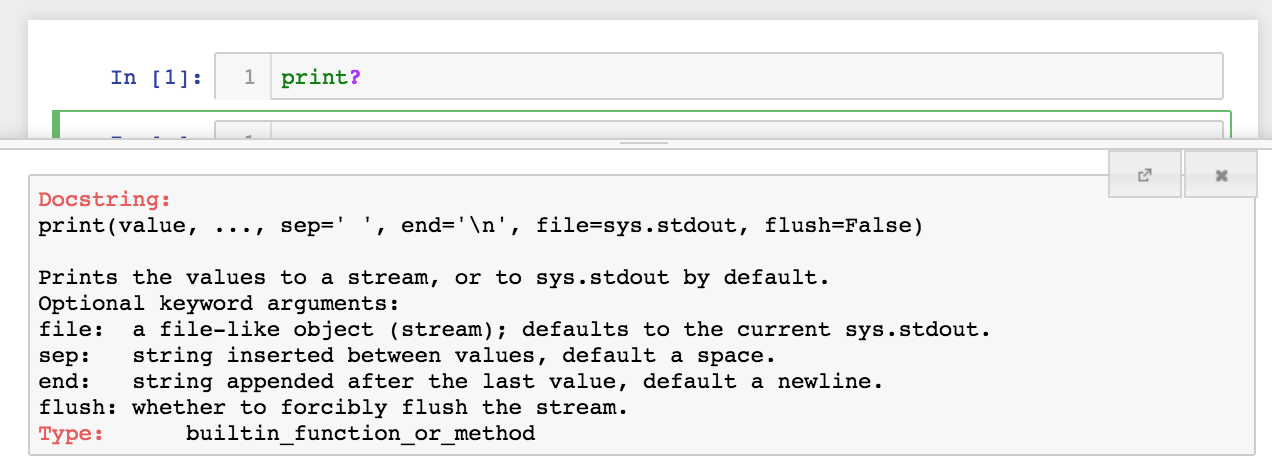
\includegraphics{images/chapter50.png}
\caption{A question mark can be used after a method or function and the
cell run in order to bring up the documentation.}
\end{figure}

Using this feature in class during live coding and modification or while
just explaining how code works helps increase student comfort and enable
them to work effectively with libraries.

\subsection{Widgets}\label{widgets}

Widgets provide the opportunity a for learners and instructors to
interact with code outputs, such as charts and tables, interactively.
Widgets are simple and quickly generated ``mini'' Graphical User
Interfaces (GUI) that give the notebook user access to slide bars,
toggle buttons, and text-boxes. They can be used in conjunction with
code, allowing a change of mindset from programming as a primary goal to
exploring a model or computation as the primary goal. Alternatively, the
code can be hidden and the widgets used to create a notebook ``app''
that might connect input parameters with a simulation and a plot.

Currently only a small subset of kernels have widget functionality. For
example, the reference implementation of widgets are the Jupyter-Python
widgets (\url{https://ipywidgets.rtfd.io}). It includes widget
components to generate and display sliders, progress bars, text boxes,
check boxes, toggle buttons, etc. Many popular visualization tools, such
as matplotlib, Plotly, leaflet.js, three.js, have Jupyter-Python widget
implementations. The documentation contains an up-to-date list of all of
the widgets and their variations. Additionally, the \texttt{interact}
method wraps allows you to wrap a function, which might be a simple
computation or a complex simulation that produces a plot, and provides
widgets for each of the inputs to the function. Figure XX shows a simple
example of a sinusoid plot whose frequency is controlled by a slide-bar.
Another kernel that has some widget functionality is C++
(\url{https://github.com/QUantStack/xwidgets}).

\begin{figure}
\centering
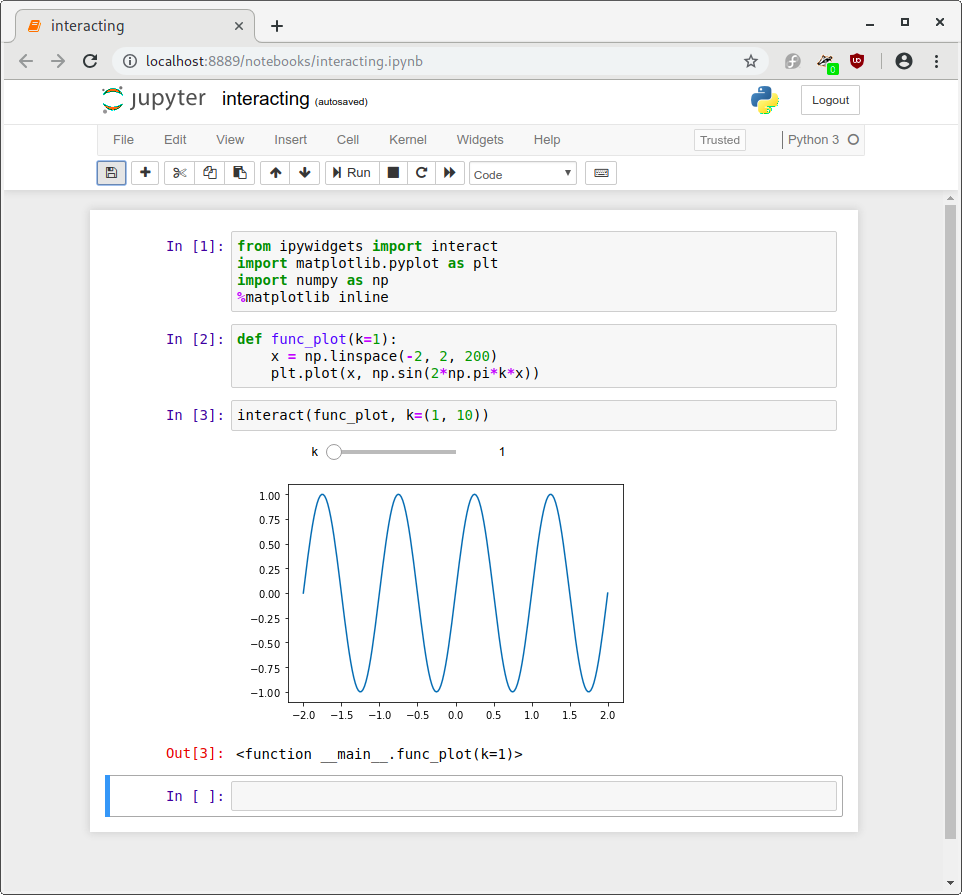
\includegraphics{images/notebook-matplotlib-interact.png}
\caption{Here, a simple slider is used to interactively change the
variable k in our function as we plot it.}
\end{figure}

In addition to the IPywidgets library, the ipyleaflet library
(\url{https://ipyleaflet.rtfd.io}) enables an interactive map to be
displayed in a notebook.

\subsubsection{Example}\label{example}

\begin{verbatim}
from ipyleaflet import Map
Map(center=[34.6252978589571, -77.34580993652344], zoom=10)
\end{verbatim}

\begin{figure}
\centering
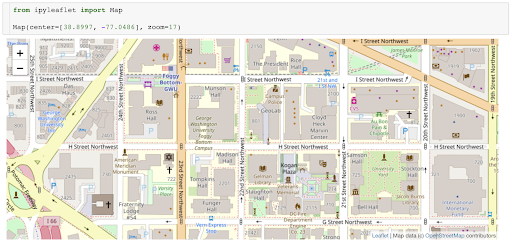
\includegraphics{images/chapter52.png}
\caption{Interactive map widget with \texttt{ipyleafletalt\_text}.}
\end{figure}

For the ambitions reader, there are resources available for you to write
your your own custom widgets. The widget cookie cutter project
(\url{https://ipywidgets.rtfd.io}) is a good place to start.

\subsection{Magics}\label{magics}

Magics are meta-commands that only function within Jupyter and allow a
user to access features that are language/kernel specific. For instance,
the IPython kernel provides a number of magics that can be useful while
developing Jupyter notebooks that uses Python as the primary language.
These are
\href{https://ipython.readthedocs.io/en/stable/interactive/magics.html}{documented}
and we will only call out a few of these here. There are many other
magics available for different kernels but the downfall of these are
that they are specific to Jupyter so does not translate to scripts and
in a teaching environment we generally recommend to be sparing in their
use so as to not obfuscate what is happening. Magics always begin with
either a single \texttt{\%} for single line commands or double
\texttt{\%\%} for applying a command to an entire cell. Many magics can
be used with single or double percents, but some do not.

\begin{itemize}
\item
  \texttt{\%run} allows for running external scripts, capturing output
  and displaying it in the notebook, e.g. \texttt{\%run\ my\_script.py}.
\item
  It is common to use matplotlib for visualization. In Jupyter, the
  magic \texttt{\%matplotlib} allows the matplotlibs resulting figures
  to be displayed in the notebook. \texttt{\%matplotlib\ inline} and
  causes static images to be embedded in the notebook and
  \texttt{\%matplotlib\ \ notebook} causes interactive images (zooming,
  panning, etc) images to be embedded.
\item
  \texttt{\%time} times the execution of the Python expression following
  the command, e.g. \texttt{\%time\ sum(range(1000))}.
\item
  \texttt{\%timeit} is is similar to \texttt{\%time} with the difference
  that it runs the expression multiple times and reports the average
  execution time.
\item
  \texttt{\%reset} removes all user defined variables along with input
  and output. Magics often have ``flags'', following the Unix command
  pattern. For example, \texttt{\%reset\ -s} is a soft reset and only
  removed user defined variables. These commands can be useful to help
  to overcome out-of-order execution problems.
\end{itemize}

A good example of a magic operating on the entire contents of cell is
the \texttt{\%\%HTML} magic that will force the cell to be interpreted
as HTML and render it appropriately. You can also use magics to call
other languages while running the IPython kernel. For example, you can
run R code from within an IPython notebook by using the \texttt{\%\%R}
magic.

\subsection{Notebooks Under Version
Control}\label{notebooks-under-version-control}

Keeping notebooks under version control is a great way to not only keep
track of changes to your created content but can also allow for sharable
content. In a course where multiple people are contributing to the
development of notebooks for the course, using version control in
conjunction with a platform like GitHub, allows authorship to be tracked
and provides communication tools for reviewing new contributions or
outlining requested development for a new assignment, activity, etc.
Another advantage of using version control is that there are services
that will provide rendered views of your notebooks that are publicly
accessible. GitHub for instance will show a rendered version of the
notebook rather than the direct text that a notebook is comprised of.
There are a few pitfalls with this with LaTeX rendering as platforms do
not always render the notebooks the same as they would appear in an
active Jupyter interface.

There are a few caveats to keeping notebooks under version control that
should be kept in mind. First of all the output will be stored in the
repository, including images, if clear output is not used before
committing changes. This can make detecting changes difficult as changes
in output will be detected when nothing has actually changed content
wise. The tracked notebooks also can become large if output is tracked.
Even with clearing the output reading through changes can be difficult
due to the format of the notebook, Notebooks are plain-text files and
the file format is represented as \href{https://www.json.org/}{JSON}.
This can be an issue if you are storing notebooks in a version control
system, like git, and you wish to see differences between versions. For
more information, see: \url{https://github.com/jupyter/nbdime} and
\url{https://github.com/mwouts/jupytext}.

\subsection{Testing Notebooks}\label{testing-notebooks}

Before distributing notebooks, and in particular if you are working with
multiple contributors to the course material, testing the notebooks
before they are distributed to students or used in a live demo can help
mitigate unexpected bugs. At a minimum, you can test that the notebook
executes cleanly from top to bottom by restarting the kernel and running
all cells from top to bottom. This can be done from the menu (Restart +
Run all).

Though it requires a bit more setup, tests can be run automatically
using a continuous integration service, such as TravisCI
(\url{https://travis-ci.org}). This will require executing the entire
notebook via the command line, for example
\texttt{jupyter\ nbconvert\ -\/-ExecutePreprocessor.enabled=True\ -\/-to=html\ my\_notebook.ipynb}
will execute the notebook (same as pressing ``Restart + Run All'') and
then convert it to HTML. These services can be connected to GitHub so
that any time that the notebooks are changed, the tests are run
automatically. Simplifying this process is an area that is under
development in the open source community. The package
\url{https://github.com/opengeophysics/testipynb} provides an easy way
to test notebooks.

\subsection{Essential Python
Libraries}\label{essential-python-libraries}

The purpose of this section is to introduce some of the most widely used
packages within the Python ecosystem. Python is not the only language
that can be used in the notebook; over 90 different kernels enable
different programming languages be used. We discuss the use of other
languages in the section:
\protect\hyperlink{using-other-languages}{Using other languages}. Python
has a large open-source community which develops and maintains an
ecosystem of over 150,000 software packages, making it a common language
of choice in many disciplines.

The core Python library
(\href{https://docs.python.org/3/}{https://docs.python.org}) contains
data types such as lists and dictionaries, as well as core functionality
such as arithmetic operators and simple file parsers. Most tasks can be
achieved with core python, however, they are often made easier with
higher-level libraries. These libraries are particularly useful for
scientific computing with Python.

Among the vast number of packages in the Python ecosystem, Numpy, Scipy,
Matplotlib and Pandas are among the most commonly used. Numpy
(\url{http://www.numpy.org/}) is a fundamental library for numerical and
scientific computing with Python. It contains data structures for
numerical arrays, tools for linear algebra, and random number
capabilities. Scipy (\url{https://docs.scipy.org/}) contains a variety
of functionality for common scientific computing tasks, such as
optimization, interpolation, statistics and signal processing. It also
includes fundamental constants from many disciplines such as the speed
of light as well as data structures for sparse matrices. Matplotlib
(\url{https://matplotlib.org/}) is the core plotting library for python
and can be used inline in the notebook with the
\texttt{\%matplotlib\ notebook} or \texttt{\%matplotlib\ inline} cell
magic. Pandas (\url{https://pandas.pydata.org/}) provides resources for
data analysis and more flexible data structures than core python. A good
resource for getting familiar with these libraries is the Scipy Lecture
Notes (\url{https://www.scipy-lectures.org}).

\subsection{Advanced topic: extensions}\label{advanced-topic-extensions}

There are many community contributed extensions that add functionality
to Jupyter notebooks. Extensions vary from displaying an automated table
of contents for a notebook, or prettify code, or hiding/showing solution
cells. Here is the link for how to install and enable extensions:
\url{https://jupyter-contrib-nbextensions.readthedocs.io/en/latest/install.html}

Here is a list of a collection of extensions that are bundled together:
\url{https://jupyter-contrib-nbextensions.readthedocs.io/en/latest/nbextensions.html}

Creating custom extensions is a way to extend or customize Jupyter to
add a capability that is not currently available with current extensions
or out of the box. These extensions may be targeted for a specific
kernel. Here are instructions for how to create and install custom
extensions:
\url{https://jupyter-notebook.readthedocs.io/en/stable/extending/frontend_extensions.html}

Figure X shows shows how Google Collaboratory, one of many tools to
interact with Jupyter notebooks, leverages the power of Jupyter
extensions for custom interaction and presentation.

\begin{figure}
\centering
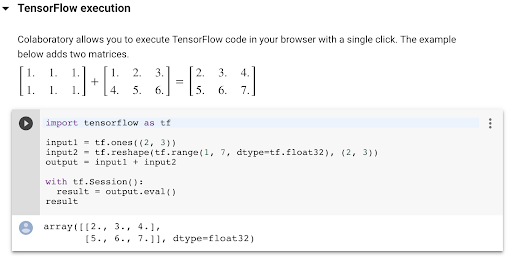
\includegraphics{images/chapter53.png}
\caption{Google Collaboratory uses Jupyter extensions to customize
Jupyter for their users. The run/play icon to the left of the code cell
is created using extensions. This is not present in the standard Jupyter
software. TensorFlow is a library for creating Machine Learning
experiments in Python.}
\end{figure}

\section{Tips and tricks}\label{tips-and-tricks}

\subsection{Reminders}\label{reminders}

If you are using a single notebook as a standalone exercise in a
traditional class (i.e., this is the only computational component of
your class), then it is helpful to have a few cells at the top of that
notebook that reviews how to navigate through the notebook and how to
insert cells, etc.

\subsection{Feedback}\label{feedback}

How do we get feedback from students in an interactive session to see if
students have completed an exercise?

A low tech solution is to give students sticky notes of different
colors, one meaning ``finished'' and one meaning ``need help'', that
they can stick on the back of their computers. The instructor can then
quickly look up to take a survey of the state of the class and decide
how to proceed.

Projecting Slack or a similar chat group on a screen and having student
copy-paste solutions (provided they are short functions) is a nice way
to let everyone in the class see one another's solutions. A positive
aspect of having multiple student solutions projected is that it can
show the variety of ways to solve a problem. This gives an opportunity
to talk about the readability of solutions and their efficiency. A
downside is that in a large class, the shear volume of posts can make it
overwhelming. Instead polling can be used to aggregate student answers
and provide some form of feedback to the instructor. Nbgrader or
travis-CI can also be options here, requiring students to submit
completed code where it is assessed automatically. These will however
require more setup and can take some time to complete.

\subsection{Explaining each cell}\label{explaining-each-cell}

A good rule of thumb is to always include a markdown cell above every
code cell.

\subsection{Custom Styling}\label{custom-styling}

New notebook creators often try to centrally manage the formatting of
headings, equations, and other textual items. For example, rather than
using a standard markdown heading, a creator may over-design the
headings by using HTML styles. This may create two problems:

\begin{enumerate}
\def\labelenumi{\arabic{enumi}.}
\item
  The rendering of the notebook markdown may change and your formatted
  HTML header may not maintain the same look over time.
\item
  Headers created using markdown can be used by notebook tools, such as
  automatically creating a Table of Contents.
\end{enumerate}

Our recommendation is to resist the desire to customize the styling and
simply use the default representations. If you want to do customization
(for example if you want to color certain cells) you can use CSS.

\subsection{Length of Notebooks}\label{length-of-notebooks}

Notebook authors sometimes make the notebooks very long with many topics
and sections. Notebook sections and cells are currently not easily
reused in a copy/paste sense for mixing intra-notebook content. Until
this functionality is available, we recommend that authors make short,
self-contained notebooks around short topics. This allows other
notebooks authors to mix and match notebooks to create curriculum.

\section{Gotchas}\label{gotchas}

\subsection{Programming Language ≠
Jupyter}\label{programming-language-jupyter}

Teaching a class entirely with Jupyter can give the sense to students
that this is the way all computational exploration is done. In
particular, students can be confused into thinking that programming
requires the notebook, instead of understanding that a notebook is just
one way to interact with a particular language. This point should be
made clear periodically. A good way to reinforce this is to show how to
take a function that has been developed and debugged in a notebook and
cut-paste it into a script (such as a file ending in .py for Python) and
then import it into the notebook to regain that functionality. Also, the
Integrated Development Environment (IDE), Spyder, has a plugin
(\url{https://github.com/spyder-ide/spyder-notebook}) that allows
notebooks to be displayed alongside Python scripts and a python terminal
which can be useful for showing this dichotomy.

\begin{figure}
\centering
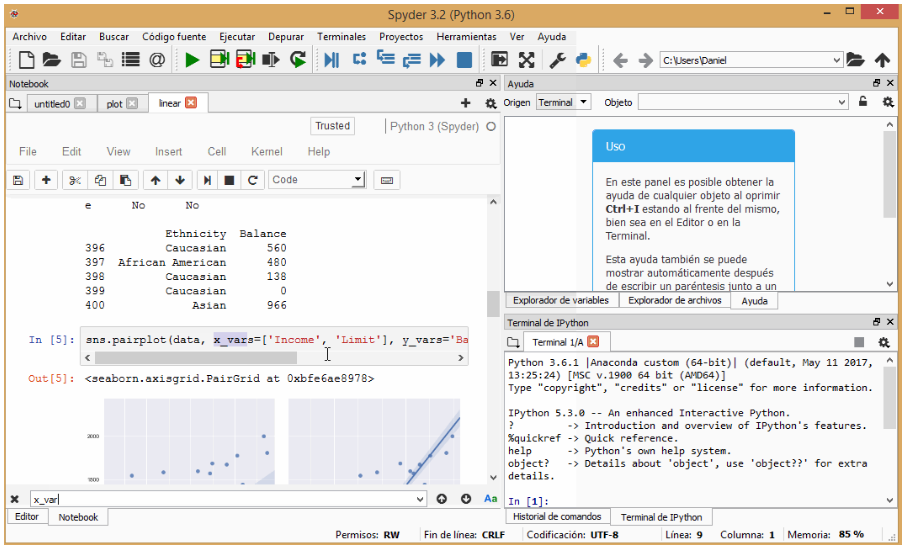
\includegraphics{images/chapter54.png}
\caption{Jupyter notebook displayed in a window pane inside Spyder.}
\end{figure}

\subsection{Restart, restart,
restart\ldots{}}\label{restart-restart-restart}

Often, students may need to stop a computation, and this can be
accomplished by pressing the ``Interrupt'' button in the toolbar.
However, students should also be made aware of how to restart the kernel
in a notebook, and what this means. There are several instances when
students might need to do this. Sometimes students write code that can
go into an infinite loop. The visual cues that notebooks give in this
case are subtle, and students may not realize this and don't understand
why the notebook is non-responsive. In live-coding situations, it can be
useful to demonstrate this to students and show them how to restart the
kernel and carry on.

A second instance of where restarting a kernel might be needed is due to
how the notebook stores the state of the computation. We like to think
that, since the notebook is laid out in a linear fashion, that the state
will always reflect what would happen if the notebook was run from the
start up to that point. However, it is common to work in a notebook out
of order, for instance if students ask a question about some previous
example. If the variable has been changed in subsequent cells, then its
value might not reflect what you expect when you rerun a cell earlier in
the notebook. Restarting the kernel is sometimes the only solution.

\subsection{Notebook hygiene}\label{notebook-hygiene}

Many gotchas can be mitigated by developing notebooks that will be
robust to incremental and non-linear execution. The main principle is to
minimize side-effects of executing a cell and manifests itself somewhat
differently in different languages; our suggestions here will be
relevant to Python and may need to be adapted for other languages.
Notebooks should generally be able to execute sequentially, such as via
``restart kernel and run all cells''. (An exception is when a notebook
is intentionally incomplete for the purpose of live coding or student
exercises, see nbgrader or the exercise estnations for more elegant ways
to handle this.) Variable mutation is the most common way in which a
notebook may malfunction when executing cells in a non-linear way (e.g.,
in response to student questions or when comparing and contrasting
different methodologies). Sometimes this mutation is incidental, through
dummy variables that were not meant to have significance outside the
scope of the cell in which they are used. Their scope can be limited by
placing them in a function, even if that function is only called once.
Redefinition of functions can often be avoided by parameterizing the
desired functionality as would typically be done if designing a library
(though this may be a distracting software design for novice
programmers). Function definitions should have little or no dependency
on variables from their enclosing scope. When modifying cells for demos
and formative assessments during class, it is useful to either copy the
cell or modify/execute such that a conforming implementation remains
present when moving on to other cells where it may be used.
Additionally, you can minimize these issues by grouping code in a single
cell that should always be executed sequentially, because code within a
cell will always be sequential.

\chapter{Getting Your Class Going with Jupyter}\label{getting-going}

You have several options on how to get Jupyter Notebooks to your
students. You can ask students to install Jupyter on their own
computers, install Jupyter on lab computers for students to use, or run
Jupyter on a remote server that your students access on the internet.

\section{Local installation on students' or lab
computers}\label{local-installation-on-students-or-lab-computers}

``Local installation'' means that each computer is running the software
that includes the Jupyter Notebook. Typically, this requires installing
a distribution that includes Jupyter, Python, and possibly other
language kernels.

A popular distribution for Jupyter is Anaconda, which is easy to install
on Windows, Mac, and Linux. Because it can install everything at the
user level, it does not require the installer to have administrator (or
root) permissions.

Two other popular open source projects that can run Jupyter notebooks
are \href{https://nteract.io/}{nteract} and
\href{https://nteract.io/atom}{Hydrogen}. nteract is installed by
downloading a binary installer from their website and double-clicking
the installation file. Once nteract is installed, any Jupyter notebook
on a student's local system can be double-clicked and it will open
within nteract. nteract's simple user interface make it an excellent
choice for students new to computer programming. Hydrogen is a
\href{https://atom.io/packages/hydrogen}{very popular plugin} for the
open source Atom editor; it's currently used by over 700,000 people.
Hydrogen lets a user edit, display, and execute a notebook within the
Atom editor.

You can ask students to install Jupyter on their own computer or make it
possible for them to use lab computers. These can also be combined: give
students the instructions to install it on their own, but also tell them
that it's available in the lab if they can't get it to work on their
laptop. This way you don't need a large enough computer lab for
everyone, and don't need to worry that not everyone can get it to work
on their own.

\subsection{Jupyter on student-owned
computers}\label{jupyter-on-student-owned-computers}

The benefits of installation on student-owned computers include:

\begin{itemize}
\tightlist
\item
  Once students have the software on their computers, they always have
  access to it; they can work anywhere, and they can use it for
  internships, jobs, and other non-school activities.
\item
  It is easy for them to install additional packages later.
\item
  Students learn to install and set up Jupyter, and software in general,
  which is a skill they are likely to need.
\item
  The total computing power for the class scales with the number of
  students, as long as each student has enough CPU power and memory to
  support the intended applications.
\item
  You can adopt Jupyter without support or resources from your
  institution.
\item
  Students learn to use Jupyter on their preferred OS, e.g.~Linux, Mac,
  or Windows, which means they are already familiar with the basic
  idioms of their OS.
\end{itemize}

Drawbacks include:

\begin{itemize}
\tightlist
\item
  This approach is only possible if every student owns a computer with
  enough capacity.
\item
  Students with less powerful computers might be at an unfair
  disadvantage.
\item
  Although installation is generally easy, it still takes time. The time
  you spend at the beginning of a class can be worthwhile for a
  semester-long course that uses Jupyter throughout, but it is a barrier
  to using Jupyter for a single module or one-off assignment in a course
  about something else.
\item
  Also, the amount of time spent debugging esoteric problems scales with
  the number of students: a class of 25 students is bound to have a few
  people with 32-bit processors, incompatible libraries, out-of-date
  operating systems, over-zealous virus checkers, etc., and a class with
  100 students will have four times as many. One work-around is to have
  students work in pairs: the probability that more than half of the
  students cannot get it working is reduced.
\item
  Discrepancies in installed library versions can cause issues for
  students and may lead to different behaviors when students run code.
\end{itemize}

Although Jupyter is cross-platform and ideally behaves the same on
Windows, Mac, or Linux, and distributions such as Anaconda also behave
very similarly on all platforms, the instructions for installing and
launching it are slightly different on each operating system, so
fine-grained instructions such as ``double click here'' or ``type this
command'' need different versions for Linux, Mac, and Windows users,
which can be challenging when the instructor presenting the material has
only one platform at their disposal. It is worth developing detailed
instructions that the students can go through at their own pace, rather
than relying only on a live demo in class that will only apply to a
fraction of the students.

\subsection{Jupyter on lab computers}\label{jupyter-on-lab-computers}

Using lab computers instead of student-owned computers has the benefits
of uniformity and improved equity. Each student will have exactly the
same setup, and the instructions will work the same for everyone. This
reduces the amount of individual tech support required and guarantees
that all students have access to enough computational power.

However, this deployment has some disadvantages:

\begin{itemize}
\item
  Depending on how much control you have of the computer lab, you might
  need institutional permission and support.
\item
  Students might be limited to working on assignments only when they are
  on campus and when computer labs are open, which might be an unfair
  disadvantage for non-resident students or those with full time jobs.
\item
  It might be difficult to install additional packages as the need
  arises, and students might not be allowed to install packages they
  need for projects.
\item
  Even in a computer lab, it can be difficult to maintain consistency
  across machines, and to keep all installations functional.

  \textbf{--- Box}

  What is Anaconda? You will see the Anaconda distribution recommended
  by many educators and course authors. Anaconda is a package manager,
  an environment manager, a Python distribution, a collection of
  \href{https://docs.anaconda.com/anaconda/packages/pkg-docs/}{over
  1,500+ open source packages}, and also Jupyter. It is free to
  download, open source, and easy to install, on any computer system
  (Windows, Mac OS X or Linux). It also includes the conda packaging
  utility to update and install new packages of the Python and R
  ecosystems, and to manage computational environments. According to the
  company's webpage, Anaconda has more than 6 million users.
  \url{https://www.anaconda.com/what-is-anaconda/} . The Software
  Carpentry project provides installation instructions with videos for
  anaconda:
  \url{https://swcarpentry.github.io/python-novice-gapminder/setup/}

  \textbf{--- Box}

  Two other popular open source projects that can run Jupyter notebooks
  are \href{https://nteract.io/}{nteract} and
  \href{https://nteract.io/atom}{Hydrogen}. nteract is installed by
  downloading a binary installer from their website and double-clicking
  the installation file. Once nteract is installed, any Jupyter notebook
  on a student's local system can be double-clicked and it will open
  within nteract. nteract's simple user interface make it an excellent
  choice for students new to computer programming. Hydrogen is a
  \href{https://atom.io/packages/hydrogen}{very popular plugin} for the
  open source Atom editor; it's currently used by over 700,000 people.
  Hydrogen lets a user edit, display, and execute a notebook within the
  Atom editor.
\end{itemize}

\section{Jupyter on remote servers}\label{jupyter-on-remote-servers}

Even when Jupyter runs locally, it runs as a web application; that is,
it runs in a browser connected to a server. In a local installation, the
browser and the server run on the same machine. But it is also possible
to run the server remotely.

In that case, students don't have to install anything; they only have to
run a browser and load a URL.

There are several ways to run Jupyter on a remote server:

\begin{enumerate}
\def\labelenumi{\arabic{enumi}.}
\tightlist
\item
  You can run Jupyter on a server owned by you or your institution.
\item
  You can run Jupyter in a temporary environment running in the cloud.
\item
  You can run Jupyter in a persistent environment running in the cloud.
\end{enumerate}

Running Jupyter remotely has many of the advantages of running in a lab:
you can provide a consistent environment and guarantee that all students
have access to sufficient computation resources. And it mitigates one of
the drawbacks of a lab installation, since students have access to cloud
resources from anywhere, not just on campus.

Working in the cloud also means that students do not have to manage
their own backups of a laptop hard drive. Although a student could still
inadvertently overwrite, delete, or destroy the contents of a notebook
stored in the cloud, they will not lose their entire work if a laptop is
damaged or lost.

For simple, one-off uses of Jupyter (say, for a single assignment or
in-class activity) the cloud option is very attractive as it requires
little in-class time to discuss installation of additional software.

\subsection{Running in a temporary environment in the
cloud}\label{running-in-a-temporary-environment-in-the-cloud}

The easiest option for running Jupyter in the cloud is to use a cloud
service that provides temporary environments. Some of these services are
free of cost, and you can use them without installing anything.

These environments are well-suited for short examples in classes that do
not use Jupyter extensively. Students can open a notebook and start
running with the push of a button.

However, there are some limitations to these services:

\begin{itemize}
\item
  If your notebooks depend on particular packages, or particular
  versions of packages, it can be difficult to satisfy these
  requirements.
\item
  These services run notebooks in a temporary environment that
  disappears if it is left idle. So they might not be suitable for
  managing student work.
\item
  Some of these services do not guarantee a level of service and may not
  be as reliable as you need for a class or workshop.

  \textbf{--- Box}

  \textbf{Binder} (\href{https://mybinder.org}{mybinder.org}) is an
  open-source service provided by Project Jupyter. It allows the owner
  of a set of notebooks residing in a git repository to pre-build an
  image in the Binder service, and get a shareable link that any visitor
  can click to obtain a working instance of JupyterHub, with the
  notebooks in the repository. The session is temporary (any changes the
  user makes will be deleted when closing the tab or window), but it's
  fully interactive. Binder is currently one of the favorite services
  for running one-off workshops or tutorials.
\end{itemize}

\subsection{Running on servers you
control}\label{running-on-servers-you-control}

If you have access to a server or cluster with enough computing power to
support your class---including CPU and especially memory---you can
provide a Jupyter as a service using JupyterHub.

JupyterHub is open-source software that provides a cloud-based Jupyter
application for each user in a group. Each user has their own account
and home directory on the server. The Hub, JupyterHub's central system,
allows authenticating users and starting individual Jupyter notebook
servers. Programs that start notebook servers can use a variety of
technical solutions. For more details, see
\url{https://github.com/jupyterhub/jupyterhub/wiki/Spawners}

Once the Hub starts a user's notebook server, the Jupyter Notebook
running in the cloud behaves just like Jupyter does when installed on an
individual's computer, but JupyterHub will be running notebooks and
storing files on a remote cloud computer. Students can download
notebooks stored in the cloud to their local computer if they wish to
work with a local installation as well. Additionally, students can
upload notebooks (and other files) from their local computer to the
cloud.

While anyone can run a JupyterHub server on their own Linux or Mac
computer, installing and configuring JupyterHub requires sophisticated
knowledge spanning the Linux/Unix operating system, system
administration, and networking. For more information, see:

\begin{itemize}
\tightlist
\item
  \url{https://github.com/jupyterhub/jupyterhub} (the basic JupyterHub
  project, which can be installed on a bare-metal server, a virtual
  private server (VPS), or a commercial cloud cluster)
\item
  \url{https://github.com/jupyterhub/the-littlest-jupyterhub} (a
  simplified installation of JupyterHub on a remote server or VPS)
\item
  \url{https://github.com/jupyterhub/zero-to-jupyterhub-k8s} (a
  step-by-step guide to install JupyterHub on a Kubernetes cloud system)
\end{itemize}

Providing a JupyterHub service offers several benefits. First, students
get up and running immediately---they spend no time installing software.
They navigate to a web URL, log in to JupyterHub, and begin using
Jupyter. This ability to quickly log in and begin computing is a
powerful way to get students to engage with the lesson, builds
confidence, and avoids the sometimes-stressful experience of installing
software on the student's computer.

However, running JupyterHub on your own server has drawbacks:

\begin{itemize}
\tightlist
\item
  Getting started is not easy; most instructors would require (or at
  least benefit from) institutional support that may not be available.
\item
  It can be difficult to scale: if the number of students increases, you
  might need more computing power. And the load students generate can be
  uneven; for example, if everyone runs a computationally-intensive
  example at the same time, your server might not be able to handle it.
\item
  This option can be expensive, unless you already have servers with
  sufficient power.
\end{itemize}

\subsection{Running Jupyter in the
cloud}\label{running-jupyter-in-the-cloud}

If you or your institution don't own computing hardware with the power
to support your class, you can run JupyterHub on virtual servers
provided by cloud services like AWS and Microsoft Azure. In those
environment, you can install JupyterHub as described in the previous
section

Commercial offerings also exist to use Jupyter in the cloud, some of
which provide free trials or a ``freemium'' pricing model. They include:

\begin{itemize}
\tightlist
\item
  CoCalc, previously MathSageCloud (\url{https://cocalc.com}) is a
  subscription service with a free trial plan. The service also includes
  the ability to share files with project collaborators. The no-cost
  version does not allow network access. This has some important
  limitations (for example, you cannot install additional packages or
  kernels).
\item
  Gryd (\url{https://gryd.us}) is another subscription service with a
  free tier. It includes course-management features, like a way to
  create a course, invite students, and deploy auto-graded assignments.
\item
  codio (\url{https://codio.com/features/ide})
\item
  Microsoft Azure notebooks (\url{https://notebooks.azure.com/} )
\item
  Amazon Sagemaker
  (\url{https://docs.aws.amazon.com/sagemaker/latest/dg/ex1-prepare.html})
\item
  Gradient by Paperspace (\url{https://www.paperspace.com/gradient})
\item
  Google Colaboratory (\url{https://colab.research.google.com/} )
\end{itemize}

The biggest advantage of these services is that they require no
installation and minimal setup by instructors, and some of them provide
features that integrate with learning management systems. However,
instructors generally have to create student accounts and set up student
environments.

These services are highly scalable; that is, they can handle large
numbers of students and uneven loads. However, they are not infallible;
they might require some tending to make sure students have access to
enough resources.

The biggest drawback of these services is that they can be expensive.
Some charge on a per-student basis, with limits on computation and
memory use. Some charge on the basis of actual use, which can be
unpredictable (and might require instructors to enforce limits on
student activities).

Other drawbacks include:

\begin{itemize}
\tightlist
\item
  It may be difficult or impossible to install packages you, or
  particular versions of packages.
\item
  Some of these services impose limits on what students can do; for
  example, they might have limited ability to access external services.
\item
  Many of these services are relatively new, and they sometimes expose
  instructors and students to rough edges.
\item
  Students generally lose access to their accounts when the class ends
  (or a limited time after).
\item
  There may be privacy concerns with sharing student information on
  commercial servers. Some institutions have agreements with one or more
  of these providers that address privacy.
\end{itemize}

\section{Distribution and Collection of
Materials}\label{distribution-and-collection-of-materials}

You may want to distribute course materials to and collect them from
students. A variety of options are available. Some important things to
consider:

\begin{itemize}
\tightlist
\item
  Do you want to share your notebooks publicly, or do they require
  privacy?
\item
  Can the notebooks that the students create or edit be public? Or do
  they require privacy?
\item
  How do you plan to assess collected notebooks?
\item
  Do you need integration with your LMS?
\item
  Do you need integration with a file-sharing system?
\item
  Do you want to distribute with the cell output showing?
\item
  Do students need software that is not easily available on their own
  (or laboratory) computers?
\end{itemize}

Jupyter notebooks are plain text computer files, so you can distribute
them to students and collect them using any system that handles text
files, including GitHub, Google Drive, and (as a last resort) email.

\subsection{Learning Management
Systems}\label{learning-management-systems}

Many instructors use a Learning Management System (LMS) to communicate
with students. These tools offer private file sharing and assignments
that connect to the students' institutional computing accounts and they
can be used to distribute and collect notebooks as text files. However,
most LMS tools are not yet notebook-aware, so they don't render
notebooks or make it easy for instructors to comment on or grade them.

Some tools and workflows are being actively developed to connect the
Jupyter ecosystem to the LMS ecosystem using the
\href{https://open.edx.org/learning-tools-interoperability}{Learning
Tools Interoperability (LTI)} standard. By the time you read this, you
might find that the options have improved.

\subsection{Web hosting}\label{web-hosting}

Notebooks can be publicly hosted on any website, so students can
download the files by clicking on a link. Most web hosting software is
not notebook-aware, but nbviewer is a web service that renders notebooks
(\url{https://nbviewer.jupyter.org/}). Also, some browser extensions can
open notebook files via nbviewer
(\url{https://github.com/jiffyclub/open-in-nbviewer}).

GitHub Pages (and other similar services) can be used to host rendered
notebooks, and continuous integration services can build the web pages
from the notebooks and then display content. See Jupyter Book
(\url{https://github.com/choldgraf/jupyter-book}) and use of
\href{https://drdoctr.github.io/doctr}{doctr} to do this.

\subsection{Git}\label{git}

One of the most popular tools for distributing and collecting notebooks
is Git, which is a version control system. Files under Git control are
often hosted on services like GitHub, GitLab, and Bitbucket. Many of
these services are notebook-aware; for example, when you view a notebook
on GitHub, you see a rendered notebook that includes formatted text,
typeset mathematics, code highlighting, and the output of the code,
including figures.

Educators at academic institutions can use GitHub Classroom, which
allows instructors to set up assignments for a class. Students click on
a link for an assignment and a copy of the assignment repo is created
and initialized with the assignment content, which can be a notebook.
Each student's repository can be made private, with access only granted
for the student and instructor. This can be an efficient way to
distribute assignments to a large class.

A drawback of Git is that it is hard to use. It might be worth spending
time in your class to teach Git if it is valuable for students to learn
about version control. But if this is not one of the learning goals for
your class, you can minimize the students' exposure to Git using
graphical interfaces like GitHub Desktop and Git for Windows.

The default Git tools for comparing files and merging changes do not
work well with Jupyter notebooks. However, there are specialized tools
to help with these tasks (see Notebooks Under Version Control).

\subsection{JupyterHub}\label{jupyterhub}

If your students are using JupyterHub, you can place notebooks and any
related files directly into the students' directories manually or via a
script. If nbgrader is available on your JupyterHub instance you can use
it to collect and distribute notebooks (whether or not you choose to use
nbgrader's assessment features). This allows you to develop the
notebooks and incrementally make them visible to the students for them
to ``fetch''. They can then edit the notebooks or create new ones in the
directory created in their storage space, and then publish their
notebooks back to you for downloading, viewing, or assessing with the
nbgrader tools (see the next section for details on this tool).

\begin{verbatim}
**— Box**


**What is nbgrader?** `nbgrader` is a tool for creating, handling, and automatically grading assignments based on Jupyter notebooks. It works as a Jupyter extension that the course creator installs on their computer. `nbgrader` is a flexible project in the Jupyter ecosystem that allows the distribution and collection of materials. As its name implies, it also can grade assignments; it can be used in a distributed manner where each student is running Jupyter on their own computers, or in a centralized manner, for example, if the students each have an account on a JupyterHub installation. (More details in the Assessment section.) <https://nbgrader.readthedocs.io>
\end{verbatim}

\subsection{Using an LMS and nbgrader
together:}\label{using-an-lms-and-nbgrader-together}

Integration of nbgrader with learning management systems is still
primitive, but the following is a strategy that works with current
tools.

\begin{enumerate}
\def\labelenumi{\arabic{enumi}.}
\tightlist
\item
  The instructor creates an assignment notebook using nbgrader, then
  distributes the assignment to students via an LMS.
\item
  Students complete the assignment and upload the solution to the LMS.
\item
  The instructor downloads the completed assignments as zip file and
  extracts the students' solutions in a Jupyter environment.
\item
  Instructors and graders use nbgrader to grade the assignment and save
  the grades to a CSV file.
\item
  The CSV file is then uploaded to the LMS.
\end{enumerate}

There are already some tools that make this workflow easier, including
the Extractor plugin to the ZipCollect feature in nbgrader
(\url{https://nbgrader.readthedocs.io/en/stable/plugins/zipcollect-plugin.html}).

\section{Assessing student learning with Jupyter
Notebooks}\label{assessing-student-learning-with-jupyter-notebooks}

Many educators develop course-assessment activities as Jupyter
Notebooks. This includes exams, in-class activities, homework
assignments, and projects.

One simple way to handle the assessment of a notebook-based submission
is to have students either print them out, email them, submit them as a
standard electronic document (say into a Course Management System), or
drop them into a shared folder. At that point, the instructor can mark
and grade them in a traditional manner, for example by simply writing
comments on a printout or adding annotations to a PDF.

\begin{verbatim}
**_Pro Tip: Printing out a notebook can sometimes result in wasted space on pages, especially for notebooks with many images or figures. Converting to PDF requires large/complex LaTeX installations. Exporting to HTML and then printing often gives a better result._**
\end{verbatim}

nbgrader allows code cells in a notebook to be marked to be auto-graded
or manually graded. An instructor can then create an assignment that can
be completely auo-graded, requiring little work after the notebook has
been created. This makes grading much easier and scales well with large
class sizes. However, creating such an auto-graded notebook in nbgrader
can be quite time-consuming. In addition, pedagogically a completely
auto-graded notebook may have serious downsides. For example, studies
suggest that students learn better when they can actively connect a
topic to their own interests {[}CITATION NEEDED{]}. One method of
encouraging this is to have a ``reflection'' question on each
submission. Such a reflection question can encourage students to comment
on the material in a personal way, but it cannot be auto-graded. Another
downside is that simply autograding code with unit tests is unlikely to
assess many of the learning objectives you might have for an assignment,
e.g., ability to use specific software-design patterns. To address this,
you can create manually graded cells for a portion of an assignment and
provide written feedback to the student.

\emph{GOTCHA: At the time of this writing, nbgrader has some limitations
that require careful use. For example, using it in a multi-class setting
(say, on JupyterHub) requires that instructors coordinate the naming of
assignments so that they do not collide.}

nbgrader is a sophisticated tool that can be set up to allow multiple
graders, teaching assistants, and more. For more information on using
nbgrader, see \url{https://github.com/jupyter/nbgrader}.

There are some third-party notebook-based assessment solutions. For
example CoCalc (\textless{}www.cocalc.com\textgreater{}) and Vocareum
(\textless{}www.vocareum.com\textgreater{}) provide a cloud notebook
platform that can also perform assessment similar to nbgrader.

\_For example, cocalc.com offers\ldots{} {[}are there other third-party
course management notebook-oriented solutions?{]} and Berkeley uses
DataHub for their large Data8 course. Vocareum
(\url{https://www.vocareum.com}) TODO

\section{How do you create Jupyter Notebooks for reuse and
sharing?}\label{how-do-you-create-jupyter-notebooks-for-reuse-and-sharing}

As you create notebooks for your lectures, computational essays, or
homework assignments, you may wish to think about how to make it
possible that they can be reused by yourself and others.

First, you may want to make the materials openly accessible and findable
via the internet. This suggests avoiding keeping the notebooks behind a
``walled garden,'' such as a Course Management System. That is, users
may have access to some material, but be prevented from seeing other
materials. You will have to decide whether you want others to have full
access. For example, many teachers do not want students to be able to
see notebooks that may have solutions, or hints of solutions and
therefore limit their access.

Callout box: To share your notebook with others you can submit it to
\url{https://www.engage-csedu.org/} This curated collection of open
educational computing resources is maintained by the National Center for
Women in Information Technology (NCWIT).

If you decide to make your notebooks reusable by others, make it clear
under which license the materials can be used. For example, you can
include a Creative Commons attribution and share-alike statement at the
bottom of your notebook. Adding a license allows people to reuse your
materials without asking for permission explicitly.
\url{https://creativecommons.org/licenses/by-sa/3.0/us/}

GitHub may be the most common service to host and share notebooks, where
they can be viewed (including rendering), downloaded, or forked by
others. (Private repositories can also be used to limit visibility to
colleagues, students, or other organizations.). Make sure to be aware of
some of the pitfalls of keeping notebooks version controlled however
(see Notebooks Under Version Control for details).

Another potential issue with sharing deals with external files that you
may want to include in your notebook. This is in contrast with content
(say a plot) that can be directly created by the notebook's code.
Possible content includes data, images and videos using code and
embedding tags in markdown or HTML. The implication is that if you share
your notebook you must include the external files along with the
notebook. This can be done a number of ways including using a version
control repository, a zip-file, or a file sharing service. Another
external dependency issue with sharing notebooks involves software
libraries. In this case you share a configuration file that a user can
use to setup the same environment. Examples of these files include a
conda env.yml, a pip requirements.txt, or dockerfile.

Because Jupyter notebooks embed the output of cells into the ipynb file
itself (e.g., images, videos, etc.), the files can grow large. To make
it possible to display the cell output via the renderers on Github,
Gitlab, or nbviewer, save the notebook after it is executed and then
upload to those services. If instead you want to reduce file size and
provide the notebooks to someone with the code cell output cleared,
choose this option in the notebook's dropdown interface. Then the user
will need to execute the notebook themselves to see the output.

\section{Jupyter: a 21st Century Genre of Open Educational Resources and
Practices}\label{jupyter-a-21st-century-genre-of-open-educational-resources-and-practices}

Educators create teaching and learning materials. With the appearance of
the internet, a community of educators began producing open access
traditional teaching materials. In parallel, a community of software
developers began creating open source software. Each community developed
their own development patterns. In particular open source software
communities gravitated to the bazaar style\footnote{The bazaar style is
  a method of collectively creating software that isn't top down
  directed like a traditional company hierarchy.} of distributed and
collaborative work. Jupyter notebooks may be the first time that these
communities are merging. Jupyter notebook authors are applying the
content creation patterns they use to the creation of open educational
resources that teach computation or teach through computation.

Open Education encompasses a large community, with its own conferences
and journals, with leaders and advocated practices. The most visible
efforts are related to Open Educational Resources (OER): the creation
and adoption of openly licensed learning materials. In 1994, Wayne
Hodgins coined the term ``learning object'' and the idea spread that
digital materials could be designed and made to be \emph{reused}. This
was followed by efforts to develop metadata standards, content
exchanges, and so on (addressing the concern of how to find the objects
to reuse them). In 1998, David Wiley coined the term ``open content''
and spread the idea that principles of Free and Open Source Software
(FOSS) could be applied to content on the World Wide Web. The Creative
Commons non-profit organization was founded in 2001 to provide
ready-made license agreements for sharing content and served a vital
infrastructure role on the spread of OER. The Creative Commons licenses
are now the most widely used licensing framework for open education. The
year 2001 also saw the launch of MIT OpenCourseWare (OCW). MIT promised
free public access for non-commercial uses of their course materials. It
was a unique commitment at an institutional level, strengthened by the
MIT brand. Other universities joined the OCW movement: Rice with the
OpenStax project (now formerly Connexion), CMU with the Open Learning
Initiative (OLI), Utah State University with the Center for Open and
Sustainable Learning, and so on. Today, the Open Education Consortium
has hundreds of members from around the world. The recurrent topics in
OER are: reducing costs for students buying textbooks, increasing
access, and dealing with copyright and licenses.

In the last few years, educators using Jupyter have been creating and
sharing all kinds of educational materials in the form of notebooks,
typically under a Creative Commons Attribution license (CC-BY). In fact,
Jupyter is \emph{a new genre of OER}. But in addition to creating open
content, educators using Jupyter often take active part in the Jupyter
community and adopt the \emph{culture} of open-source software. This is
a culture with strong ethical commitments, related to freedom of access,
transparency, and governance (Coleman, 2012). The content they create
has the value of giving access (the very definition of OER), under an
open model. But open-source culture also promotes a culture of
collaboration. In this regard, engaging in teaching with Jupyter opens
new possibilities for educators to engage in \emph{open development} and
collaborate with others in producing lessons, tutorials, courses, and
even books.

REF---Coleman, E.G., 2012. Coding freedom: The ethics and aesthetics of
hacking. Princeton University Press.

NOTE from Carol: Installation on a student computer or web-based access.
Installation on computer lab computers or web-based access. Web-based
access requires additional decisions and system administration
resources.

\section{Notes}\label{notes}

\chapter{Usage Case Studies}\label{case-studies}

Contributors to this chapter: you may increase adoption by new users if
you integrate information about some of the following into your case:

\begin{enumerate}
\def\labelenumi{\arabic{enumi}.}
\tightlist
\item
  Demonstrate that you can increase students' ability to:

  \begin{enumerate}
  \def\labelenumii{\arabic{enumii}.}
  \tightlist
  \item
    Engage material \& participate in class
  \item
    Understand material and perform well
  \item
    prep their for career
  \item
    Enjoy learning this way
  \end{enumerate}
\item
  describe:

  \begin{enumerate}
  \def\labelenumii{\arabic{enumii}.}
  \tightlist
  \item
    how it fits with how their students learn
  \item
    how it connects to how they teach
  \item
    the needed resources (support, hardware, etc.)
  \item
    the necessary logistics (e.g., how much time will it take? Be
    honest: time is a consideration, and an important reason that people
    do not adopt new practices, but is not a reason that they stopped
    using one)
  \item
    what Jupyter does in terms of promoting learning, instructor
    affordances
  \end{enumerate}
\end{enumerate}

\section{Jupyter Notebooks in Support of Scaling for Large
Enrollments}\label{jupyter-notebooks-in-support-of-scaling-for-large-enrollments}

\subsection{Supporting large enrollment courses at UC
Berkeley}\label{supporting-large-enrollment-courses-at-uc-berkeley}

The University of California at Berkeley started a pilot course titled
``Foundations in Data Science'' (also known as Data-8) for about 100
incoming undergraduate students in Fall 2015. Data-8, the fastest
growing course in Berkeley's history, is entirely Jupyter-based,
allowing the program to scale the course to 1,400 students in 2018. This
scale is made possible by Jupyter's shared computational environment. In
particular, Jupyter allowed ``browser-based computation, avoiding the
need for students to install software, transfer files, or update
libraries'' (see The Course of the Future and the Technology Behind It
{[}\url{https://data.berkeley.edu/news/coursefuture}{]}). Data-8 is
powered by JupyterHub and all the course materials are published openly
(\url{http://data8.org}).

\subsection{Large-scale adoption: Jupyter across
Canada}\label{large-scale-adoption-jupyter-across-canada}

Recognizing the importance of data science, computational research, and
educational resources, the \href{https://www.pims.math.ca/}{Pacific
Institute for the Mathematical Sciences (PIMS)}, in partnership with
\href{https://www.computecanada.ca/}{Compute Canada} and
\href{https://www.cybera.ca/}{Cybera}, have launched JupyterHub
platforms (under the project name Syzygy) to support researchers and
educators across Canada. Syzygy (\url{http://syzygy.ca}) provides access
to cloud-hosted Jupyter resources using existing institutional
credentials and encourages the development of computational and data
science skills. It is currently accessible at 16 institutions across the
country (McMaster, Queen's, SFU, UAlberta, UBC, UCalgary, ULethbridge,
UNewBrunswick, UOttawa, URegina, USask, UToronto, UVic, UWashington
(US), UWaterloo, Yorku) and has been used by over 11,000 people at those
institutions.

Syzygy is extensively used for teaching, but is also being used for
research activities. One notable example is a scientific software
seminar at the University of British Columbia, where graduate students
and post-doctoral researchers meet to share and learn data science
techniques with their peers. Initiatives are also underway, as part of
syzygy, to deepen its relevance into research by providing seamless
access to larger and more varied types of resources (GPUs, parallel
machines, different language kernels etc.).

Callysto (\url{https://callysto.ca/}) is a related project, also
launched by PIMS and Cybera, to bring Jupyter to students in Canadian
middle and high schools (grades 5-12). Callysto focuses on creating and
curating open content (\url{https://github.com/callysto}). This content
forms the basis of project workshops, where teachers can work through
the materials interactively, before taking them back to their
classrooms. The content links to a supporting JupyterHub installation
(integrated with the authentication systems for the networks of school
districts) allowing easy access to the materials and a Jupyter
environment to learn and create in.

-- Ian Allison

\subsection{Quick switch: moving an existing course to Python and
Jupyter (at the last
minute)}\label{quick-switch-moving-an-existing-course-to-python-and-jupyter-at-the-last-minute}

For many years, our chemical engineering kinetics course had used
software for differential equation and nonlinear simultaneous equation
solving to simulate reactors and solve design problems. The software,
recommended and described by the textbook, was installed in the
college's computer labs, but licenses for student-owned computers were
expensive and it was only available for Windows. In Spring 2015, I was
informed my class now had 52 students, but the largest computer lab had
room for only 40. As the semester progressed and we neared the chapters
that required numerical simulation, I rewrote the examples using Python
and SciPy and created Jupyter Notebooks, walking students through the
steps involved in setting up and solving the problems. I found Lorena
Barba's open-source MOOC materials online, and adapted these for my
``getting started'' notebooks. I had students install Anaconda on their
own computers, and got everyone up and running without any central
infrastructure or support from the college's IT staff. I found the
Jupyter Notebook format of including ``lecture note'' style commentary
along with short, unintimidating, snippets of code, to be extremely
effective. A couple of years later I passed on the course to a new
instructor, who took my course materials, taught himself some Python,
and continued to use Jupyter Notebooks for content delivery and
assignments.

The first year was a bit rough around the edges as I introduced it quite
late in the semester. Still, it is clear that the approach resonated
with students. An alumnus from my 2016 course wrote, ``I thought that
your course was very successful, especially the use of Jupyter Notebook
as a classroom and assignment tool. I still remember specific problems
that we went over in class (e.g., the microfluidic reactor array with
heterogeneous catalysis), and I feel that the use of Python to solve
problems throughout the course greatly benefited my understanding of
fundamental concepts. I went on to use Python {[}in the pharmaceutical
industry{]}, where I built tools for bioinformatics data analysis,
mutation network profiling for protein engineering experiments, and RNA
structure prediction from experimental data and molecular
thermodynamics.''

-- Richard West

\section{\texorpdfstring{The ``CFD Python'' story: Guiding Learners at
their Own
Pace}{The CFD Python story: Guiding Learners at their Own Pace}}\label{the-cfd-python-story-guiding-learners-at-their-own-pace}

``CFD Python'' is a collection of Jupyter Notebooks based on a practical
module that I began using in class in my Computational Fluid Dynamics
(CFD) course at Boston University in 2009. The 5-week module develops
worked examples that build on each other to incrementally guide the
learner to create a program to solve the Navier-Stokes equations of
fluid mechanics, in 12 steps. In 2013, I was invited to teach a
mini-course in the Latin-American School in High-Performance Computing,
in Argentina. The Jupyter Notebooks platform allowed me to create a
guided narrative to support learners with different background
experience and knowledge. For that event, we wrote IPython Notebooks
based on the CFD course module, to use as instructional scaffolding in
the 2-full-days of minicourse. Twenty students worked through the
notebooks as self-paced lessons, while I went from desk to desk asking
and answering questions. About four of the students completed all the
lessons in the 2 days, a bulk of them achieved up to about Step 8, and a
few of them lagged behind in Steps 4 or 5 by the end of the course. For
those who completed the full module, they had achieved in 2 days what my
regular students in the classroom normally took 5 weeks to do. Seeing
that was an eye-opening moment: both the power of worked examples in
code, and the ability to allow learners to follow their own pace made a
remarkable difference in these learners.

\emph{REF --- Barba, Lorena A., and Forsyth, Gilbert F. (2018). CFD
Python: the 12 steps to Navier--Stokes equations. Journal of Open Source
Education, 1(9), 21, \url{https://doi.org/10.21105/jose.0002} }

Based on the experience developing the ``CFD Python'' learning module,
we adopted this basic design pattern for creating lessons using
computable content:

\begin{enumerate}
\def\labelenumi{\arabic{enumi}.}
\tightlist
\item
  Break it down into small steps
\item
  Chunk small steps into bigger steps
\item
  Add narrative and connect
\item
  Link out to documentation
\item
  Interleave easy exercises
\item
  Spice with challenge questions/tasks
\item
  Publish openly online
\end{enumerate}

-- Lorena A. Barba

\section{Analyzing Music with
music21}\label{analyzing-music-with-music21}

I became interested in learning more about Python in 2013 after reading
a tutorial by Luciano Ramalho as he was writing Fluent Python. Since I
tend to seek out projects that match my outside interests (music, art,
and nature) I was looking for Python projects with music and came across
Myke Cuthbert's music21 project. Music21, an open source music theory
and analysis library maintained by Professor Michael Cuthbert at MIT,
provides a set of tools to answer questions about music quickly and
simply. Users can create, analyze, and share music with just a few lines
of code. Myke's use of the Notebook hooked me. Unlike many things that I
had worked on before, the notebooks made it easy to get started and to
write small code snippets that did real work! The more I used the
notebooks and showed them to people that I taught at Fab Lab San Diego,
the more that I saw the power of the notebook to engage a user and
empower them to explore and learn.

Music, a universal language, appeals to learners of all origins, ages,
education levels, and interests. As a subject that casts a wide appeal,
music offers the opportunity to engage and delight learners. It's an
accessible subject that has a low barrier to entry for learners from
disciplines beyond computer science and engineering.

-- Carol Willing

\textbf{Education Benefits}

\begin{itemize}
\tightlist
\item
  lessons notebooks can be tailored to age appropriate content within
  music
\item
  multisensory
\item
  ability in K12 to align with the standards
\item
  possibilities for bringing in multi-subject learning

  \begin{itemize}
  \tightlist
  \item
    writing
  \item
    history
  \item
    math
  \item
    science
  \end{itemize}
\item
  accessibility through audio and braille
\end{itemize}

\textbf{Misc quotes (perhaps pick a couple?):}

\emph{``I think of music21 as being composed of two parts. The first is
infrastructure, routines for reading, writing, and manipulating musical
scores, while the second consists of a higher-level analytical
toolkit---generating a Roman numeral from a chord and key, putting
chords into normal form, checking for parallel fifths, identifying
scales containing a given pitch or chord, and so on.'' ---Bruce
Tymoczko, Professor of Music, Princeton}

Inclusive

\emph{``It's not exclusive, but inclusive, which is the whole spirit of
jazz.'' --- Herbie Hancock}

Education

\emph{``So, you can't stay in one place, no matter how comfortable that
place is. It's all about growing.''---Mavis Staples}

Universal

\emph{``Music in the soul can be heard by the universe.''---Lao Tzu}

Communication

\_Music is the greatest communication in the world. Even if people don't
understand the language that you're singing in, they still know good
music when they hear it.``---Lou Rawls\_

\emph{``In the beginner's mind there are many possibilities. In the
expert's mind there are few.'' --Shunryu Suzuki}

\section{Interactivity in Computer Science (high school and middle
school)}\label{interactivity-in-computer-science-high-school-and-middle-school}

\textbf{Who}

High school and middle school students at Cal Poly SLO's EPIC program
completed a two hour workshop on Interactivity in Computer Science. The
workshop participants included dual language learners (English as a
Second Language) and students who have had limited access to computers
prior to the workshop.

\textbf{Why}

Providing early access to at-risk groups who may not see themselves as
capable of learning to code or use computation

Illustrate that there are many skills beyond math and science that are
needed to create software applications

\textbf{What}

Two hour workshop that maximizes ``hands on'' exploration with the goal
of building an ongoing interest in computer science

\begin{itemize}
\tightlist
\item
  short lectures

  \begin{itemize}
  \tightlist
  \item
    interactive discussion - LISTEN
  \item
    hands on - DO/APPLY This section is self-paced to engage different
    learning styles and prior knowledge
  \item
    recap - DISCUSS
  \end{itemize}
\item
  8 or so projects with achievements outlined
\item
  modern curriculum including p5.js, jupyter, binder, deep learning and
  machine learning with TensorFlow and Magenta (art and music)
\item
  Goal is to empower students to understand that they CAN use CS to
  solve real world problems
\end{itemize}

Instructor Approach

\begin{itemize}
\tightlist
\item
  Start with high quality engaging content
\item
  Self contained notebooks
\item
  Use widgets to add additional interactivity
\end{itemize}

\section{Interactive geophysics with
Jupyter}\label{interactive-geophysics-with-jupyter}

The GeoSci.xyz project (\url{https://geosci.xyz}) is an effort to
develop a community of scientists and educators around learning
resources and software for the geosciences. The project includes
multiple open-source textbooks, each which have associated Jupyter
notebook ``apps'' that serve as interactive simulation engines for
exploring concepts in geophysics. We have used these resources in an
undergraduate course on applied geophysics at the University of British
Columbia; this course is primarily taken by by geologists and engineers
(non-geophysics majors). In 2017, we delivered a 2 day short course for
professionals, graduate students, and researchers in 26 different
countries around the world (\url{https://disc2017.geosci.xyz}). In both
of these courses, the goal is to provide learners with an overview of
the various geophysical methods (e.g.~magnetics, gravity, seismic,
electromagnetics) and concepts governing the physics; we do not dive
into details of the math nor do we expect students to program or write
any lines of code. The role of Jupyter notebooks in these courses is to
serve as a tool for visualizing and exploring the physics.

During a lecture, the notebooks as a presentation medium lend to a
dynamic presentation style, where we as instructors can select model
parameters based on student input. Concepts are reinforced as students
then use these same notebooks in labs and assignments. We have found
that the notebook apps are most effective when students are first asked
to critically think about what they expect to see and then visualize the
result. If the resultant image matches their expectation, then they
understand the concept, and if not, it is an opportunity to learn and
further explore.

TODO ! {[}alt\_text{]} (images/Chapter-70.png ``image\_tooltip'')

\textbf{Caption: Notebook ``app'' for exploring the direct current
resistivity experiment over a two layer earth
(\url{https://em.geosci.xyz/apps.html}). }

-- Lindsey Heagy

\section{Investigating Hurricanes}\label{investigating-hurricanes}

\textbf{Who }

Middle school and high school students visiting Columbia's School of
Engineering and Applied Sciences on a field trip

\textbf{Why }

Students often come through looking to tour labs and experience some of
the research that is being done at the school. Unfortunately certain
fields, in this case computational mathematics and hurricane research,
do not lend themselves to these types of events.

\textbf{What }

Instead of a lab or lecture a computer lab was reserved for an hour and
a Jupyter notebook used to walk students through some basic
visualizations and data analysis encouraging students to change the code
displayed to answer questions such as ``Where did Hurricane Sandy go?''
and ``What storms occurred during 1981?''. This includes a number of
visualizations of hurricane tracks, coloring by strength of storms, and
an analysis of average number of storms per year. Notebook is available
at \url{https://github.com/applied-math/demos}.

-- Kyle T. Mandli

TODO ! {[}alt\_text{]} (images/Chapter-71.png ``image\_tooltip'')

\textbf{Fig: }Visualization from the notebook at
\url{https://github.com/applied-math/demos} demonstrating the paths of
Atlantic hurricane tracks from 1950-2012 with coloring demonstrating
category of storm.

\chapter{About the Authors}\label{authors}

\section{Project Lead}\label{project-lead}

\subsection{Lorena A. Barba}\label{lorena-a.-barba}

\begin{itemize}
\tightlist
\item
  George Washington University
\item
  \href{mailto:labarba@email.gwu.edu}{\nolinkurl{labarba@email.gwu.edu}}
\item
  \href{https://twitter.com/LorenaABarba}{@LorenaABarba}
\end{itemize}

Lorena A. Barba is Associate Professor of Mechanical and Aerospace
Engineering at the George Washington University. She adopted Jupyter in
2013 and since then used it in every course she teaches. Her open course
materials are well known and used by thousands of learners:
\href{http://lorenabarba.com/blog/cfd-python-12-steps-to-navier-stokes/}{CFD
Python} and
\href{https://github.com/numerical-mooc/numerical-mooc}{Numerical MOOC}
are the best examples.

\section{Authors at the sprint}\label{authors-at-the-sprint}

\subsection{Lecia J. Barker}\label{lecia-j.-barker}

\begin{itemize}
\tightlist
\item
  University of Colorado Boulder
\item
  \href{mailto:lecia.barker@colorado.edu}{\nolinkurl{lecia.barker@colorado.edu}}
\item
  \href{https://twitter.com/leciab}{@leciab}
\end{itemize}

\href{https://www.colorado.edu/cmci/people/information-science/lecia-barker}{Lecia
Barker} is an Associate Professor and Associate Chair of Undergraduate
Studies in the
\href{https://www.colorado.edu/cmci/infoscience}{Department of
Information Science} at the University of Colorado Boulder. She is also
a Senior Research Scientist for the
\href{https://www.ncwit.org/}{National Center for Women \& IT}. Her
research group is studying the
\href{https://csteachingpractices.wordpress.com/}{diffusion and adoption
of teaching practices} in undergraduate computer science. Lecia holds a
Ph.D.~in Communication from CU Boulder and an MBA in Marketing from San
Diego State University.

\subsection{Douglas Blank}\label{douglas-blank}

\begin{itemize}
\tightlist
\item
  Bryn Mawr College
\item
  \href{mailto:dblank@brynmawr.edu}{\nolinkurl{dblank@brynmawr.edu}}
\item
  \href{https://twitter.com/dougblank}{@dougblank}
\end{itemize}

\href{https://cs.brynmawr.edu/~dblank/}{Douglas Blank} is Associate
Professor in the \href{https://cs.brynmawr.edu/}{Department of Computer
Science} at \href{http://brynmawr.edu/}{Bryn Mawr College}, a small,
all-women's college outside of Philadelphia, PA, USA. He has a joint
Ph.D.~in Cognitive Science and Computer Science from Indiana University,
Bloomington. For over 20 years, Douglas has taught all levels of
Computer Science. For the last 4 years, he has used Jupyter notebooks
exclusively in the classroom. Douglas has published in the areas of
Computer Science Education, Robotics, Artificial Intelligence, and Deep
Learning. He is on the advisory board of
\href{https://www.engage-csedu.org}{Engage-CSEdu.org}, a joint project
between Google and the National Center for Women and Information
Technology (NCWIT). Douglas also writes text and code at his website
\href{http://douglasblank.com}{douglasblank.com}.

\subsection{Jed Brown}\label{jed-brown}

\begin{itemize}
\tightlist
\item
  University of Colorado Boulder
\item
  \href{mailto:jed@jedbrown.org}{\nolinkurl{jed@jedbrown.org}}
\item
  \href{https://twitter.com/five9a2}{@five9a2}
\end{itemize}

\href{https://jedbrown.org/}{Jed Brown} is an Assistant Professor of
Computer Science at the University of Colorado Boulder. He has been
teaching numerical and scientific computing courses using Jupyter
Notebook and nbgrader for three years, and leads a research group that
develops computational methods and community software for computational
science.

\subsection{Allen Downey}\label{allen-downey}

\begin{itemize}
\tightlist
\item
  Olin College
\item
  \href{mailto:downey@allendowney.com}{\nolinkurl{downey@allendowney.com}}
\item
  \href{https://twitter.com/AllenDowney}{@AllenDowney}
\end{itemize}

\href{http://www.allendowney.com/wp/}{Allen Downey} is a professor of
Computer Science at Olin College and the author of a series of
open-source textbooks related to software and data science, including
\emph{Think Python}, \emph{Think Bayes}, and \emph{Think Complexity},
published by O'Reilly Media. These books, and the classes based on them,
use Jupyter notebooks extensively. Prof Downey holds a Ph.D.~in computer
science from U.C. Berkeley, and M.S. and B.S. degrees from MIT.

\subsection{Tim George}\label{tim-george}

\begin{itemize}
\tightlist
\item
  Project Jupyter
\item
  \href{mailto:tgeorgeux@gmail.com}{\nolinkurl{tgeorgeux@gmail.com}}
\end{itemize}

\href{https://www.tgeorgeux.com/}{Timothy George} is the Lead UI/UX
Designer for \href{https://jupyter.org/}{Project Jupyter}, focusing
primarily on JupyterLab. In addition to his formal duties, Tim is also
in working with Jupyter on design strategy, future products, governance,
diversity and inclusion. He studied HCI at UC Irvine's Donald Bren
School of Informatics and Computer Science where he received a Master's
Degree.

\subsection{Lindsey Heagy}\label{lindsey-heagy}

\begin{itemize}
\tightlist
\item
  University of California Berkeley
\item
  \href{mailto:lindseyheagy@gmail.com}{\nolinkurl{lindseyheagy@gmail.com}}
\item
  \href{https://twitter.com/lindsey_jh}{@lindsey\_jh}
\end{itemize}

\href{https://www.lindseyjh.ca/}{Lindsey Heagy} is a Postdoctoral
Researcher at the University of California Berkeley working on Project
Jupyter and Jupyter in the geosciences. She recently completed her PhD
at the University of British Columbia in geophysics. She is a project
leader of \href{http://geosci.xyz}{GeoSci.xyz}, an effort to build
collaborative, interactive, web-based textbooks in the geosciences, and
a core contributor to \href{https://www.simpeg.xyz/}{SimPEG}, an open
source framework for geophysical simulation and inversions. The
GeoSci.xyz project relies heavily on Jupyter for making the content come
to life.

\subsection{Kyle Mandli}\label{kyle-mandli}

\begin{itemize}
\tightlist
\item
  Columbia University
\item
  \href{mailto:kyle.mandli@columbia.edu}{\nolinkurl{kyle.mandli@columbia.edu}}
\item
  \href{https://twitter.com/KyleMandli}{@KyleMandli}
\end{itemize}

\href{https://www.columbia.edu/~ktm2132}{Kyle Mandli} is an Assistant
Professor in the Department of Applied Physics and Applied Mathematics
at Columbia University. He has developed a set of openly available
course notes centered around Jupyter notebooks and uses Jupyter for
homework in conjunction with nbgrader. His other research interests
include development of computational methods for coastal hazards such as
storm surge and tsunamis.

\subsection{Jason K. Moore}\label{jason-k.-moore}

\begin{itemize}
\tightlist
\item
  University of California, Davis
\item
  \href{mailto:jkm@ucdavis.edu}{\nolinkurl{jkm@ucdavis.edu}}
\item
  \href{https://twitter.com/moorepants}{@moorepants}
\end{itemize}

\href{http://moorepants.info/}{Jason K. Moore} is an Assistant Teaching
Professor of Mechanical and Aerospace Engineering at the University of
California, Davis. He currently teaches dynamics and mechanical design
related courses. He utilizes Jupyter notebooks to teach modeling and
simulation and is working on a
\href{https://moorepants.github.io/resonance}{textbook about Mechanical
Vibrations}. He is responsible for the Jupyter related features in the
\href{http://libretexts.org}{LibreTexts project} and is also a core
developer of the \href{http://sympy.org/}{SymPy} and
\href{http://pydy.org/}{PyDy} projects which utilizes Jupyter for
training workshops, e.g.
\href{https://www.sympy.org/scipy-2017-codegen-tutorial/}{PyDy Tutorial}
and \href{https://github.com/pydy/pydy-tutorial-human-standing}{SymPy
Code Generation Tutorial}. Jason has PhD, MSc, and BSc degrees in
mechanical engineering from UC Davis and Old Dominion University.

\subsection{David Lippert}\label{david-lippert}

\begin{itemize}
\tightlist
\item
  Leidos
\end{itemize}

David Lippert is a software engineer at
\href{https://www.leidos.com}{Leidos} in Arlington, Virginia. He
utilizes Jupyter notebooks primarily for exploratory data analysis and
for training and evaluating machine learning algorithms. He has written
Jupyter notebooks to create new Dr.~Seuss sonnets and to evaluate if the
\href{https://www.rottentomatoes.com/about}{Rotten Tomatoes Tomatometer}
can be trusted. He has a BA in computer science from Middlebury College.

\subsection{Kyle Niemeyer}\label{kyle-niemeyer}

\begin{itemize}
\tightlist
\item
  Oregon State University
\item
  \href{mailto:kyle.niemeyer@oregonstate.edu}{\nolinkurl{kyle.niemeyer@oregonstate.edu}}
\item
  \href{https://twitter.com/kyleniemeyer}{@kyleniemeyer}
\end{itemize}

\href{https://niemeyer-research-group.github.io/}{Kyle Niemeyer} is an
Assistant Professor of Mechanical Engineering in the School of
Mechanical, Industrial, and Manufacturing Engineering at Oregon State
University. He teaches courses in numerical and analytical methods for
solving differential equations as well as gas dynamics, and recently
developed a
\href{https://softwaredevengresearch.github.io/syllabus/}{graduate
course on software development for engineering research}. His research
group develops and applies methods for modeling combustion and
chemically reacting fluid flows. He is also on the steering committee of
the \href{https://cantera.org/}{Cantera} open-source project for
chemical kinetics, thermodynamics, and transport processes.

\subsection{Ryan Watkins}\label{ryan-watkins}

\begin{itemize}
\tightlist
\item
  George Washington University
\item
  \href{mailto:rwatkins@gwu.edu}{\nolinkurl{rwatkins@gwu.edu}}
\item
  \href{https://twitter.com/parsingscience}{@parsingscience}
\end{itemize}

\href{https://gsehd.gwu.edu/directory/ryan-watkins}{Ryan Watkins} is a
Professor of Educational Technology at George Washington University in
Washington DC. He leads the
\href{https://go.gwu.edu/phd}{Human-Technology Collaboration (HTC)} PhD
program area, and he teaches courses in needs assessment, instructional
design, and research methods. Ryan's research focuses on how people and
organizations define and assess needs. He is co-host of
\href{https://parsingscience.org/}{Parsing Science}, a podcast where
researchers share the stories behind their science. He also developed
the \href{https://wesharescience.org/}{We Share Science} platform for
sharing video abstracts of research.

\subsection{Richard West}\label{richard-west}

\begin{itemize}
\tightlist
\item
  Northeastern University
\item
  \href{mailto:R.West@northeastern.edu}{\nolinkurl{R.West@northeastern.edu}}
\item
  \href{https://twitter.com/richardhwest}{@richardhwest}
\end{itemize}

\href{https://web.northeastern.edu/comocheng/}{Richard West} is
Associate Professor of Chemical Engineering at Northeastern University
in Boston. He leads a research group in computational modeling for
complex reacting systems like combustion or catalysis. He is a core
member of the \href{https://cantera.org/}{Cantera} open-source project.
As well as in an elective on ``computational modeling in chemical
engineering'', he has integrated Python and Jupyter into core classes on
chemical kinetics and reactor design, at both the undergraduate and
graduate levels. As part of his NSF CAREER award, he is developing
modules to teach students to use Python and SciPy to solve chemical
engineering problems.

\subsection{Elizabeth Wickes}\label{elizabeth-wickes}

\begin{itemize}
\tightlist
\item
  University of Illinois at Urbana-Champaign
\item
  \href{mailto:wickes1@illinois.edu}{\nolinkurl{wickes1@illinois.edu}}
\item
  \href{https://twitter.com/elliewix}{@elliewix}
\end{itemize}

\href{https://ischool.illinois.edu/people/elizabeth-wickes}{Elizabeth
Wickes} is a Lecturer at the School of Information Sciences at the
University of Illinois at Urbana-Champaign. She teaches foundational
programming from an information and data sciences perspective, as well
as other coursework on open data and reproducibility. Her programming
course lectures are written in Jupyter Notebooks and the class is taught
via live coding.

\subsection{Carol Willing}\label{carol-willing}

\begin{itemize}
\tightlist
\item
  Cal Poly San Luis Obispo
\item
  \href{mailto:willingc@gmail.com}{\nolinkurl{willingc@gmail.com}}
\item
  \href{https://twitter.com/WillingCarol}{@WillingCarol}
\end{itemize}

\href{https://www.willingconsulting.com/about/}{Carol Willing} is a
Research Software Engineer at Cal Poly San Luis Obispo working full-time
on \href{https://jupyter.org/}{Project Jupyter}. She is a Python
Software Foundation Fellow and former Director; a Project Jupyter
Steering Council member; and a core developer on CPython and Jupyter.
Carol has an M.S. in Management from MIT and a B.S.E. in Electrical
Engineering from Duke.

\subsection{Michael Zingale}\label{michael-zingale}

\begin{itemize}
\tightlist
\item
  Stony Brook University
\item
  \href{mailto:Michael.Zingale@stonybrook.edu}{\nolinkurl{Michael.Zingale@stonybrook.edu}}
\item
  \href{https://twitter.com/Michael_Zingale}{@Michael\_Zingale}
\end{itemize}

\href{http://www.astro.sunysb.edu/mzingale/}{Michael Zingale} is an
Associate Professor and computational astrophysicist at Stony Brook
University. He has a PhD from University of Chicago (2000). He
frequently teaches
\href{http://bender.astro.sunysb.edu/classes/numerical_methods/}{numerical
methods} and
\href{http://bender.astro.sunysb.edu/classes/python-science/}{Python for
scientific computing} graduate courses, relying on Jupyter notebooks and
python for much of the presentation. He is an advocate for open
educational resources, as a founder of the
\href{https://github.com/Open-Astrophysics-Bookshelf/}{Open Astrophysics
Bookshelf project} where he hosts his
\href{http://bender.astro.sunysb.edu/hydro_by_example/CompHydroTutorial.pdf}{\emph{Introduction
to Computational Astrophysical Hydrodynamics}} text.

\chapter{Glossary}\label{glossary}

\textbf{Anaconda}: a free, open-source package manager, environment
manager, Python distribution, and collection of
\href{https://docs.anaconda.com/anaconda/packages/pkg-docs/}{over 1,500+
open source packages} including and also Jupyter.
\url{https://www.anaconda.com/what-is-anaconda/}

\textbf{API (Application Programming Interface)}: the exact details of
interacting with software, usually used by other software.

\textbf{Binder}: a hosted service that allows anyone to launch their own
sandboxed notebook environment from a Git repository.
\url{https://mybinder.org}

\textbf{cell}: the area in a Jupyter Notebook where you can enter
markdown, or computer code.

\textbf{cloud, in the}: used to describe software or documents hosted on
a remote computer accessed over the internet.

\textbf{CSV (Comma Separated Values)}: referring to a comma-separated
value file. A plain-text file format such that each line is a list of
data separated by commas.

\textbf{execute}: technical term for having the computer perform the
instructions of your program. Alias for ``run it.''

\textbf{extension, Jupyter}: in this instance, it is not a request for
more time. Rather, a Jupyter extension is a bit of code, often developed
by a third-party, that adds additional functionality to Jupyter. For
example, a popular extension is a Table of Contents creator.

\textbf{flipped classroom}: a teaching style where students work on
their own outside of class to learn new material (sometimes by watching
recorded lectures or reading descriptive/interactive notebooks) and the
come together in the classroom to practice what they've learned through
exercises or experiments.

\textbf{Git}: a popular version control system (VCS) used for keeping
track of changes of files over time.

\textbf{IDE (Integrated Development Environment)}: software that assists
in the development of additional software.

\textbf{Jupyter}: The term ``Jupyter'' may refer to one of a couple of
different things: a community of users and developers focused on the
open source software; the collection of tools and standards that,
together, allow projects like the Jupyter Notebook to operate. The name
refers to the three core programming languages supported: Julia, Python,
and R.

\textbf{JupyterHub}: a cloud service that can provide access to Jupyter
notebooks and environments to multiple users via a modern web browser.
\url{http://jupyter.org/hub}

\textbf{kernel}: In Jupyter, a kernel is the packaging up of a language,
and related programs needed to run it. For example, Python2 and Python3
are separate kernels.

\textbf{LMS (Learning Management System)}: a cloud service that helps
instructors manage aspects of classrooms.

\textbf{load}: how many students can a computer support?

\textbf{Markdown}: a text format that allows for basic formatting
(headers, text styles, links) mixed inline with the text. Markdown files
usually have the extension \texttt{.md} and can be rendered natively by
GitHub and other tools.

\textbf{magic}: a meta-command typically starting with one or two
percent signs. Changes the meaning of the contents of a line (one
percent sign, \texttt{\%}) or the cell (two percent signs,
\texttt{\%\%}) from code to a particular meta-instruction. For example,
\texttt{\%\%R} indicates that the cell contents will be interpreted as
commands to the R language. Magics are kernel-specific (e.g., vary with
the kernel in use).

\textbf{nbgrader}: a tool for creating, handling, and automatically
grading assignments based on Jupyter notebooks.
\url{https://nbgrader.readthedocs.io}

\textbf{nbviewer}: a web application for rendering Jupyter notebooks as
static web pages, providing a URL to share and view them with a modern
web browser. \url{https://nbviewer.jupyter.org}

\textbf{nbconvert}: a tool for converting Jupyter notebooks into other
formats such as PDF, HTML, LaTeX, Markdown, reStructuredText, and
others. \url{https://nbconvert.readthedocs.io}

\textbf{notebook hidden state}: a technical term referring to the value
of variables that may have surprising results due to cells having been
executed in a non-sequential order.

\textbf{open source}: software and documents that are created in a
manner that give you rights to be able to use, and reproduce.

\textbf{pattern}: A ``pattern'' is a technical term referring to an
abstract description of a labeled process. For example, ``wash, rinse,
repeat'' is a common pattern for cleaning various objects.

\textbf{service, JupyterHub}: JupyterHub can take advantage of
additional separate, but integrated, software extensions. These are
called ``services.''

\textbf{script}: a colloquial term for a computer program.

\textbf{unit test}: a technical term for a ``test'' for checking to see
if software is operating correctly.

\textbf{URL (Universal Resource Locator)}: the address of a resource
(e.g., webpage) on the internet.

\textbf{widget}: a user interface (such as buttons, sliders, and
checkboxes) that allow the easy control of hidden computer code.

\bibliography{book.bib}


\end{document}
